\documentclass[aspectratio=169,10pt]{beamer} \mode<presentation>
\usetheme[numbering=fraction]{Boadilla}
\setbeamertemplate{navigation symbols}{}

% --- Fonts & math (LuaLaTeX) ---
\usepackage{fontspec}
\usepackage{mathtools}     % load before unicode-math
\usepackage{unicode-math}
\unimathsetup{
  warnings-off = {
    mathtools-overbracket,
    mathtools-colon
  }
}

\setsansfont{TeX Gyre Heros}
\setmonofont{JetBrains Mono}
\setmathfont{Latin Modern Math}

\usepackage{bookmark}
% Examples of Beamer-native tweaks
%\setbeamertemplate{enumerate items}[default]  % numbers
%\setbeamertemplate{itemize items}[triangle]   % bullets

\setbeamertemplate{items}[ball]
\setbeamertemplate{blocks}[rounded][shadow=true]


% --- Extras ---
\usepackage{siunitx}
\usepackage{graphicx}
\usepackage{tikz}
\usetikzlibrary{arrows.meta,positioning,calc}
\usepackage{hyperref}
\hypersetup{colorlinks=true, urlcolor=blue!70!black, linkcolor=blue!60!black, pdfpagemode=FullScreen}

% ---- Graphics path
\graphicspath{{figs/}}

% ---- Title info ----
\title{NVH, a walk down memory lane}
\subtitle{by an old applied mathematician}
\author{H\aa vard Vold}
\institute{Vold LLC}
\date{October 8-10, 2025}

% ---- Handy macros (examples) ----
\newcommand{\R}{\mathbb{R}}
\DeclareMathOperator*{\argmin}{arg\,min}

\begin{document}

% ===== Title slide =====
\maketitle

% ===== Outline =====
\section[Outline]{}
\frame{\frametitle{Outline} \tableofcontents}

\AtBeginSection[] {
  \begin{frame}{Next topic}
    \tableofcontents[currentsection]
  \end{frame}
}

% ===== Section 1 =====
% \section{Motivation}

% \begin{frame}{Problem Statement}
% \begin{itemize}
%   \item Concise bullet point with \alert{highlight}.
%   \item Another point with a small math example:
%     \[
%       f(x) = \frac{1}{\sqrt{2\pi\sigma^2}} e^{-\frac{(x-\mu)^2}{2\sigma^2}}
%     \]
% \end{itemize}
% \end{frame}

% \begin{frame}{Two-Column Layout}
% \begin{columns}[T,onlytextwidth]
%   \begin{column}{0.52\textwidth}
%     \textbf{Left:} bullet list
%     \begin{itemize}
%       \item Key idea A
%       \item Key idea B
%     \end{itemize}
%   \end{column}
%   \begin{column}{0.44\textwidth}
%     \textbf{Right:} figure
%     \begin{figure}
%       \centering
%       
\includegraphics[width=\linewidth]{logo.png}% replace with your file
%       \caption{Example figure.}
%     \end{figure}
%   \end{column}
% \end{columns}
% \end{frame}

% % ===== Section 2 =====
% \section{Method}

% \begin{frame}[t]{Theorem/Proof (numbered)}
% \begin{block}{Theorem}
% Let $A\in\R^{n\times n}$ be symmetric positive definite. Then it has $n$ positive eigenvalues and admits a Cholesky factorization.
% \end{block}

% \begin{exampleblock}{Sketch of Proof}
% Use the spectral theorem for real symmetric matrices. For the factorization, apply induction or standard constructive proofs.
% \end{exampleblock}
% \end{frame}

% \begin{frame}{Displayed Math and Steps}
% We minimize
% \[
%   \argmin_{x\in\R^n} \; \tfrac12\|Ax-b\|_2^2 + \lambda\|x\|_1.
% \]
% \pause
% Using a proximal gradient step:
% \[
%   x^{k+1} = \mathrm{soft}\bigl(x^k - \tau A^\top(Ax^k-b),\, \tau\lambda\bigr).
% \]
% \end{frame}

% \begin{frame}{TikZ Diagram}
% \centering
% \begin{tikzpicture}[node distance=1.6cm]
%   \tikzstyle{box}=[draw,rounded corners,inner sep=6pt,align=center]
%   \node[box] (a) {Input $x$};
%   \node[box,right=of a] (b) {$A$};
%   \node[box,right=of b] (c) {Output $y_{\aleph}=A^H_{\alpha}\tilde{x}$};
%   \draw[-{Latex[length=3mm]}] (a) -- (b);
%   \draw[-{Latex[length=3mm]}] (b) -- (c);
% \end{tikzpicture}
% \end{frame}

% ===== Section 3 =====
\section{Modal Testing}
\subsection{Multiple Exciter Locations}


\begin{frame}
  \begin{figure}
    \centering
    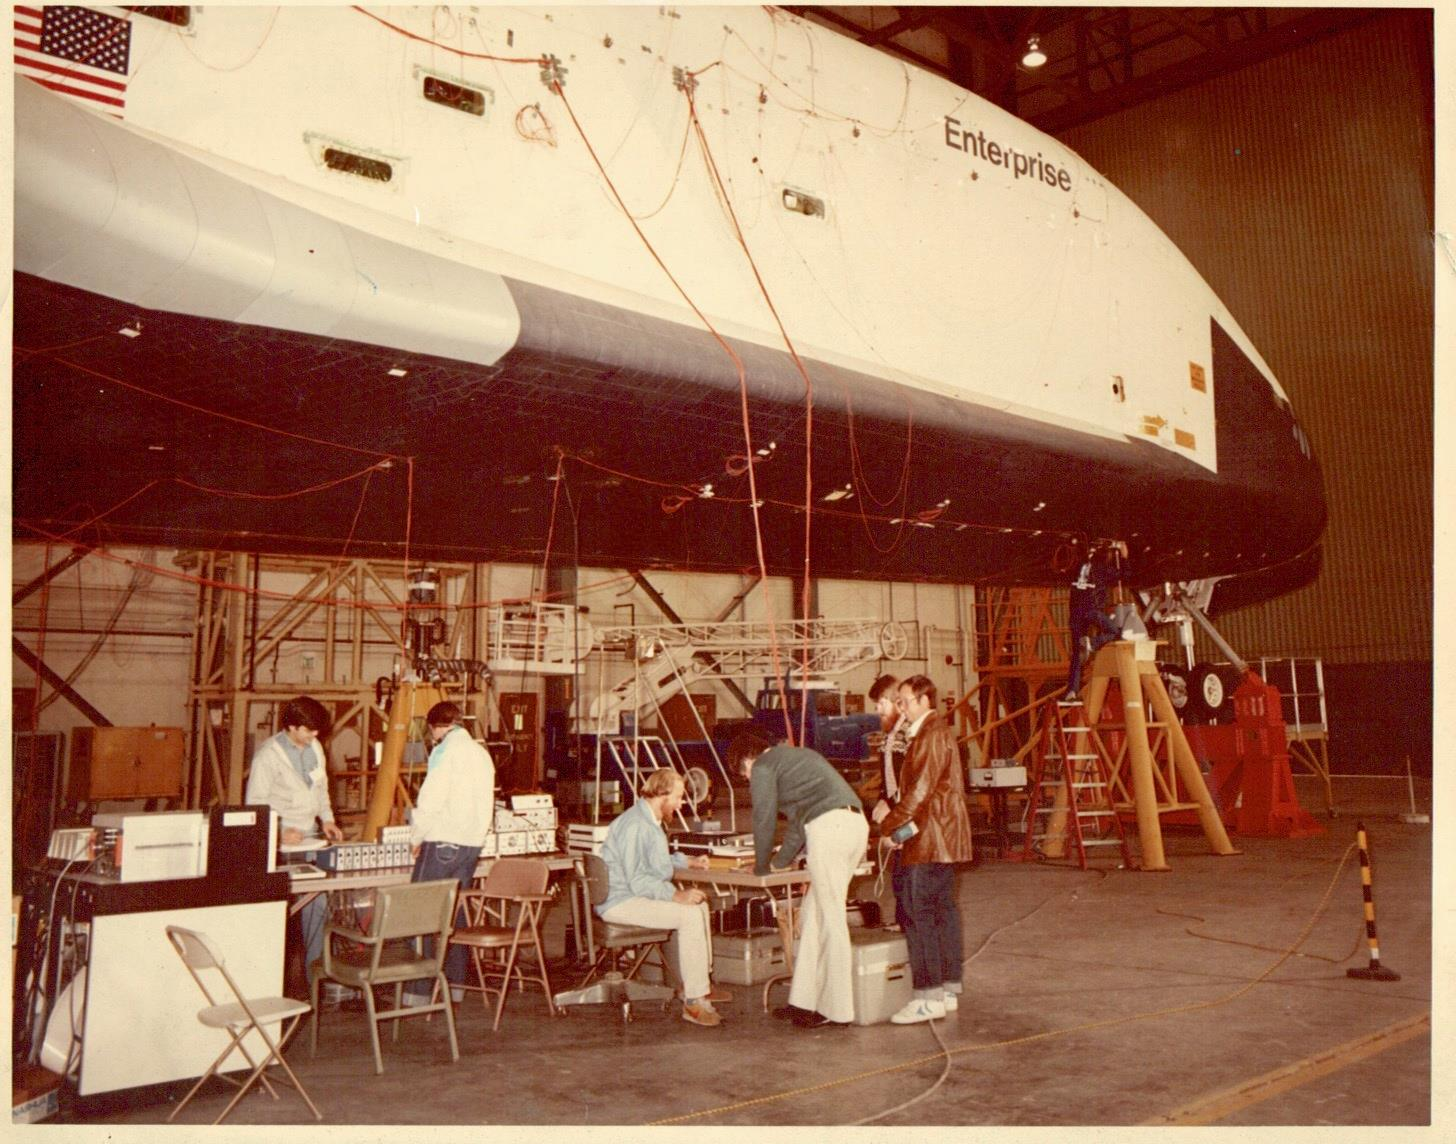
\includegraphics[width=0.65\linewidth,height=7cm]{SDRC-shuttle-1983}
    \caption{Shuttle GVT at Edwards AFB, 1983}
  \end{figure}
\end{frame}

\begin{frame}
  \begin{figure}
    \centering
    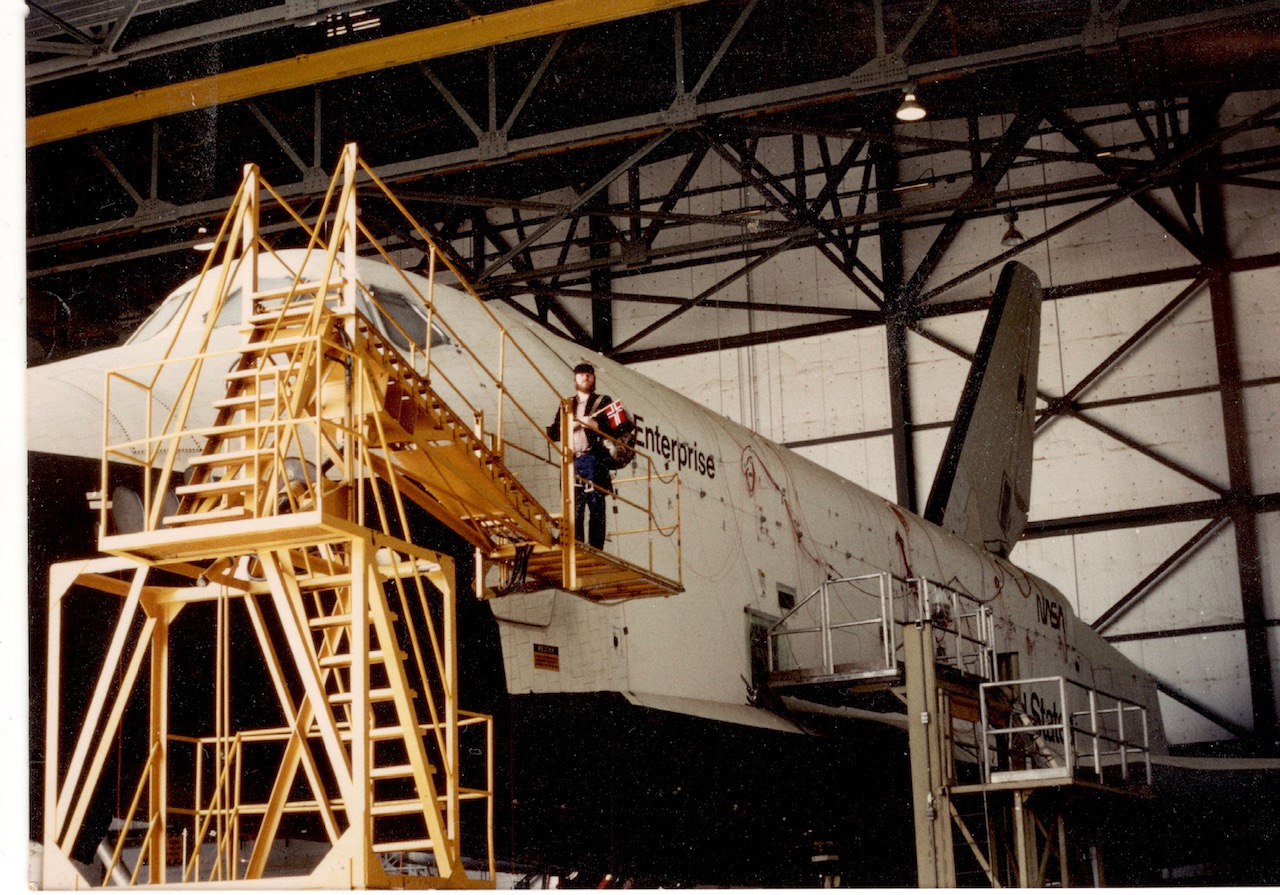
\includegraphics[width=0.65\linewidth,height=7cm]{Shuttle-1983}
    \caption{Claiming the Shuttle Orbiter Vehicle for Norway, 1983}
  \end{figure}
\end{frame}

\begin{frame}
  \begin{figure}
    \centering
    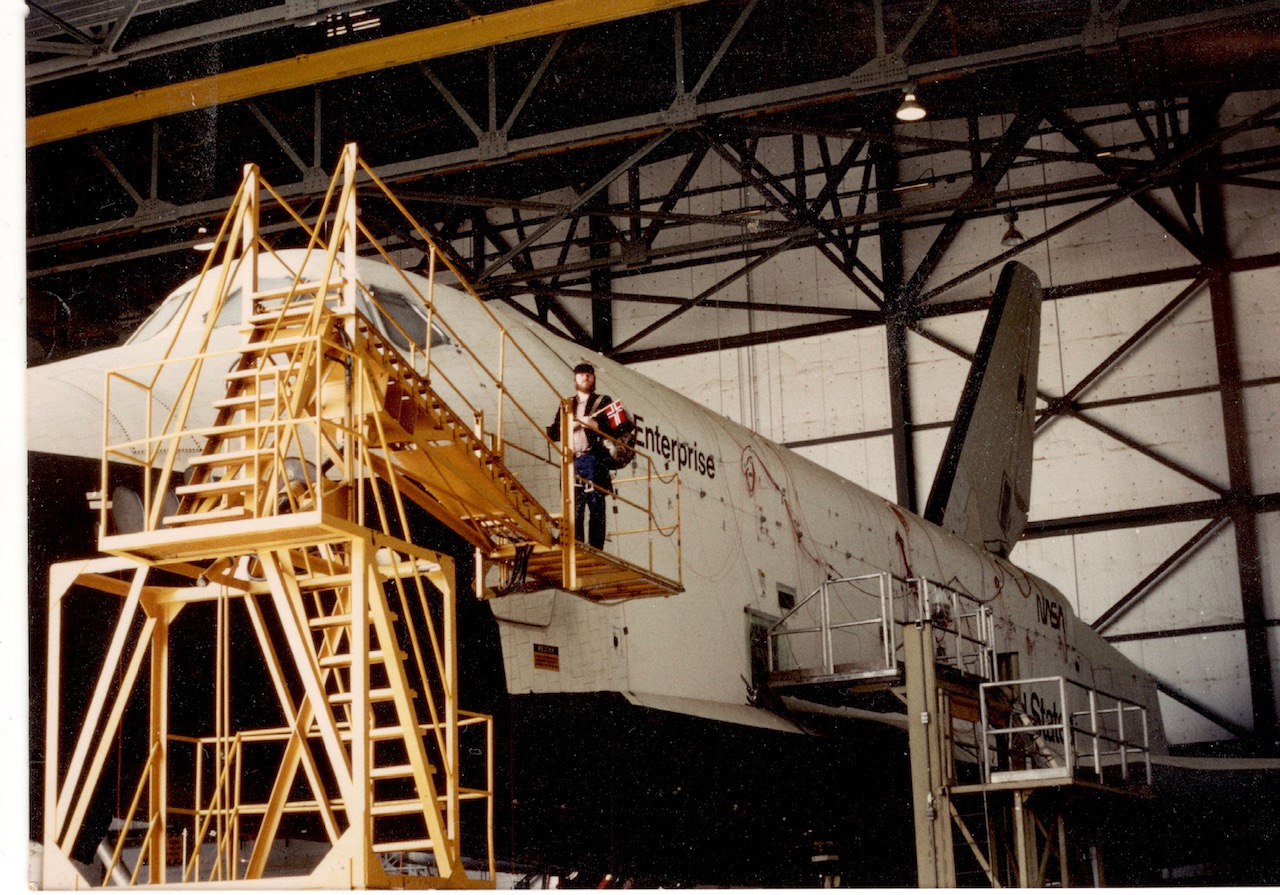
\includegraphics[width=0.65\linewidth,height=7cm]{Shuttle-1983}
    \caption{Claiming the Shuttle Orbiter Vehicle for Norway, 1983}
  \end{figure}
\end{frame}
\begin{frame}{Figure with Caption and Reference}
\begin{figure}
  \centering
  
\includegraphics[width=0.7\linewidth]{logo.png}
  \caption{Performance vs. size.}
  \label{fig:perf}
\end{figure}
As seen in Fig.%~\ref{fig:perf}, the method scales sublinearly.
\end{frame}

\begin{frame}{Side-by-Side Lists}
\begin{columns}[T,onlytextwidth]
  \begin{column}{0.48\textwidth}
    \textbf{Pros}
    \begin{itemize}
      \item Simple
      \item Fast
      \item Robust
    \end{itemize}
  \end{column}
  \begin{column}{0.48\textwidth}
    \textbf{Cons}
    \begin{itemize}
      \item Needs tuning
      \item Assumes convexity
    \end{itemize}
  \end{column}
\end{columns}
\end{frame}

%adding in the old material
 
\section{Spacecraft Cabin Ventilation Fan in NASA Glenn Acoustical Test Laboratory}
\frame{\frametitle{Spacecraft Cabin Ventilation Fan in Acoustical Test Lab}
  Microphone array traverses 168\,inches at 1\,inch/second continuously.\\
  Fan runs at 12,000\,RPM. 9 blades in rotor.
  \begin{columns}[t]
    \column{0.3\textwidth}
    \begin{figure}
      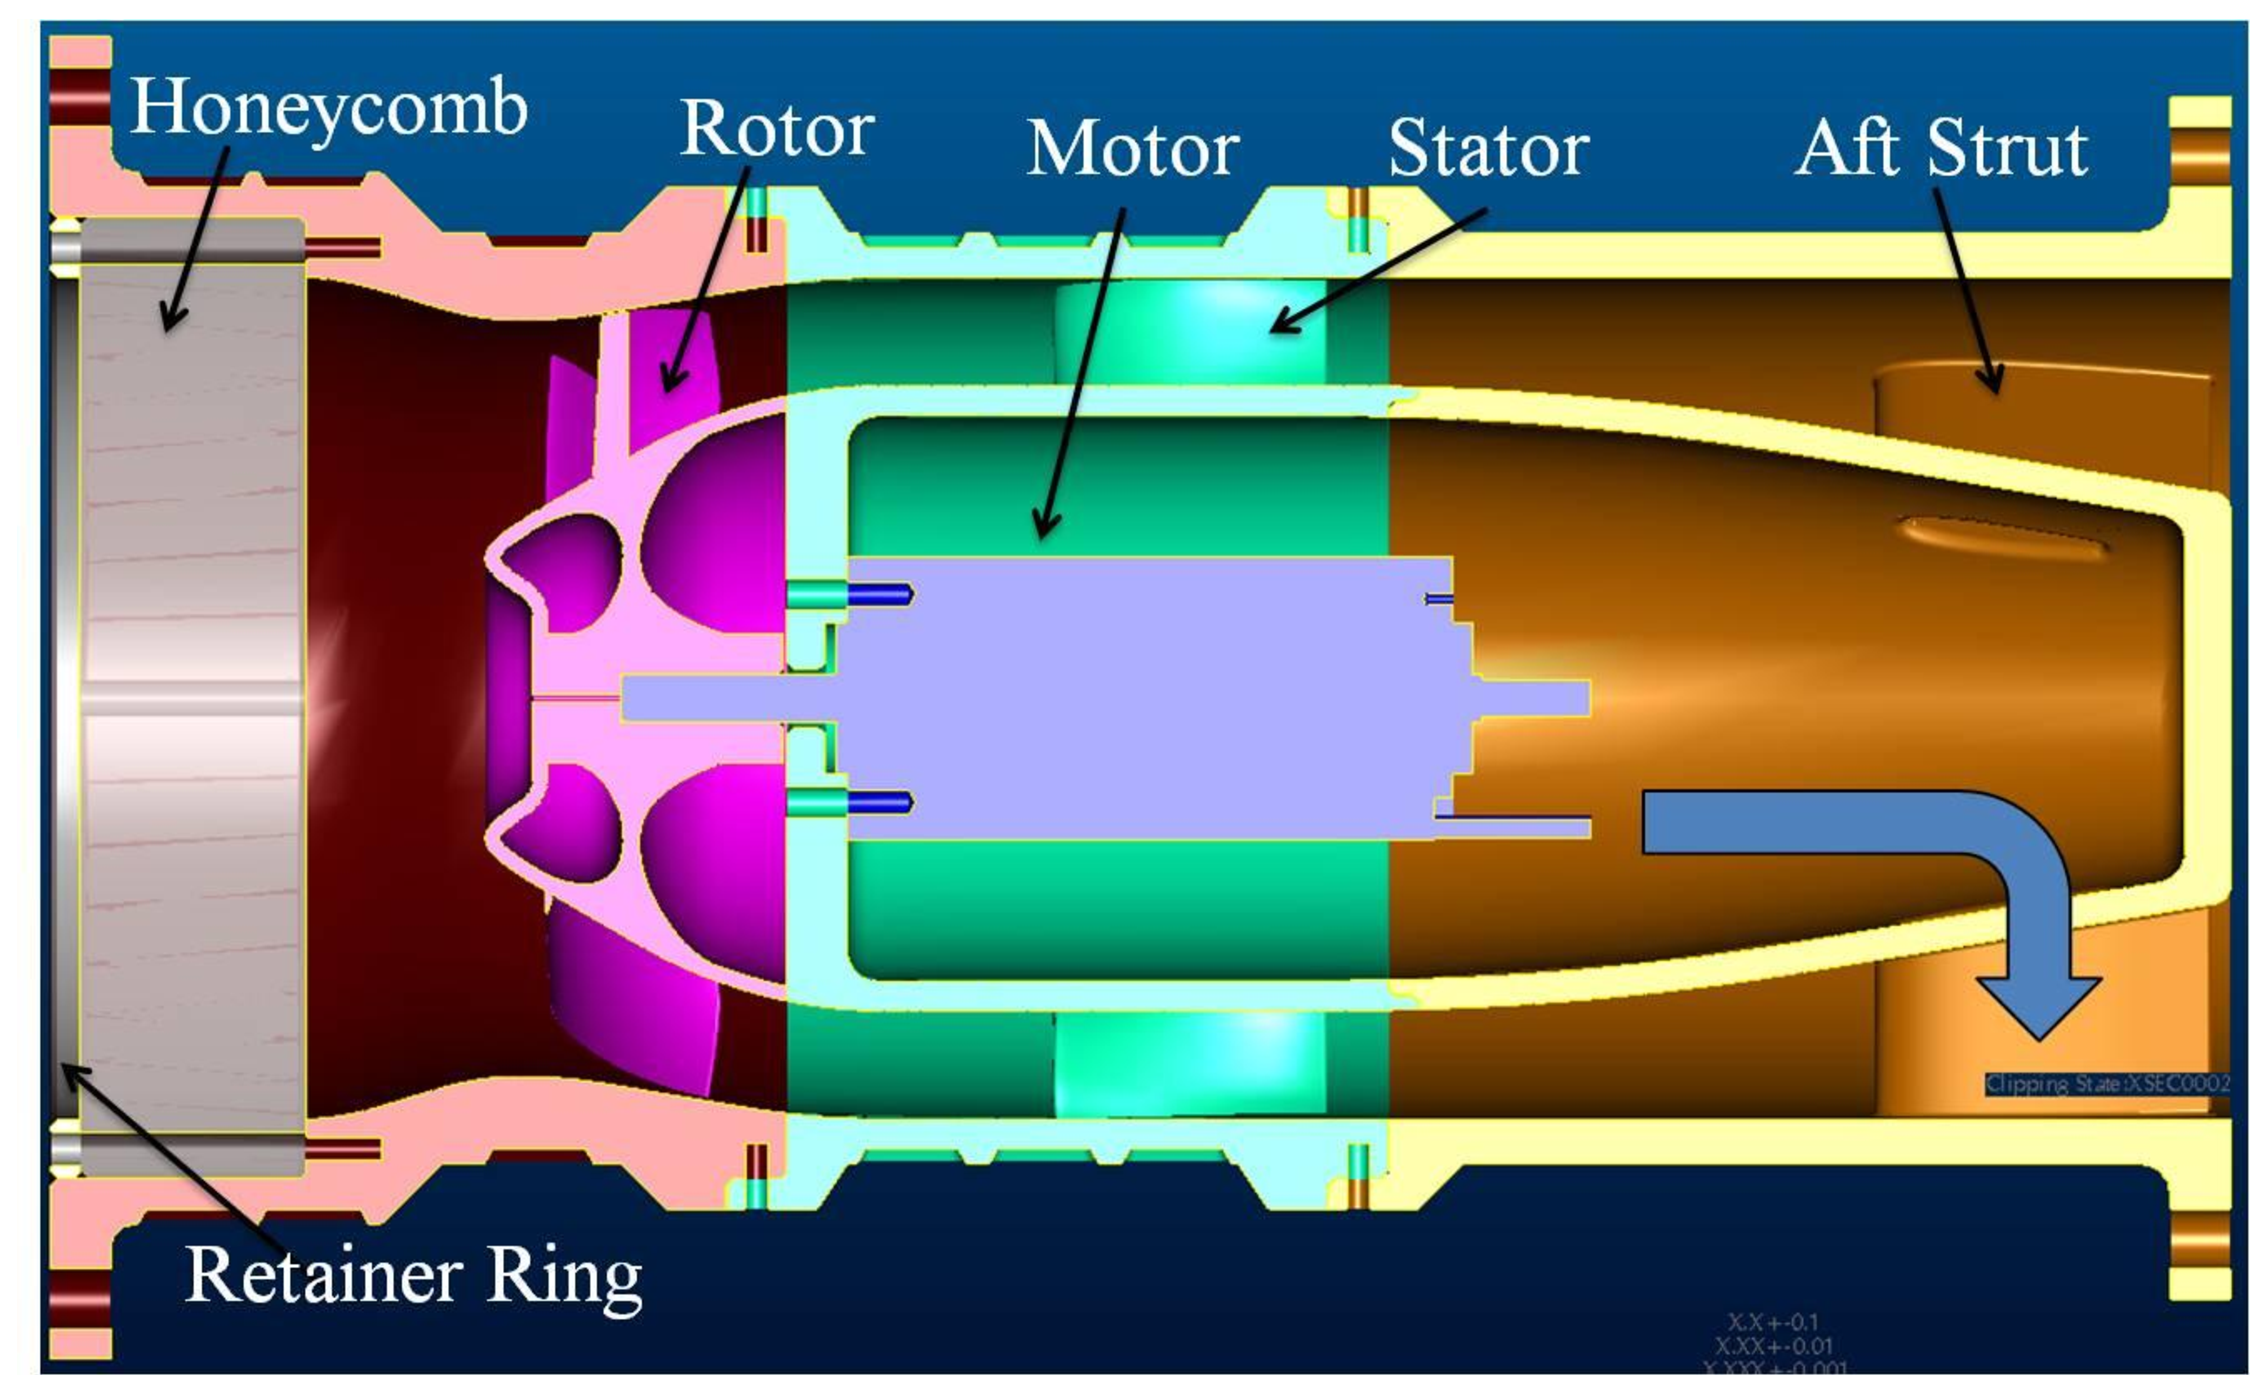
\includegraphics[width=3cm]{Spacefan03262012}
    \end{figure}
    \begin{figure}
      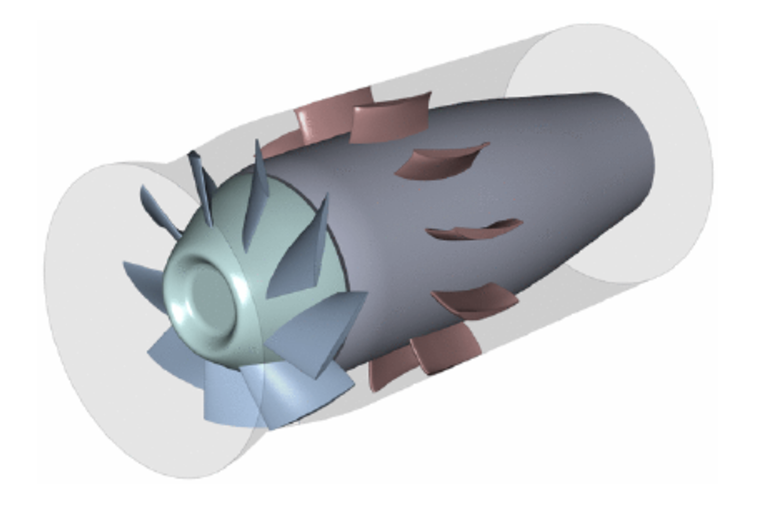
\includegraphics[width=3cm,trim=0 40 0 0]{VentFanAeroDesign}
    \end{figure}
    Fan size 9 by 4\,inches \column{0.7\textwidth}
    \begin{figure}
      \includegraphics[width=7cm,trim=0 20 0 80]{2011_04416_300}
    \end{figure}
  \end{columns}
}

\frame{\frametitle{POD of 4 Stationary Microphones (principal spectra)} 
  Blade passes 1, 2
  and 3 at 1.8\,kHz, 3.6\,kHz and 5.4\,kHz generate \emph{self-coherent} sound
  fields. Several \emph{mutually incoherent} broadband sound fields in each frequency
  band.
  \begin{figure}
    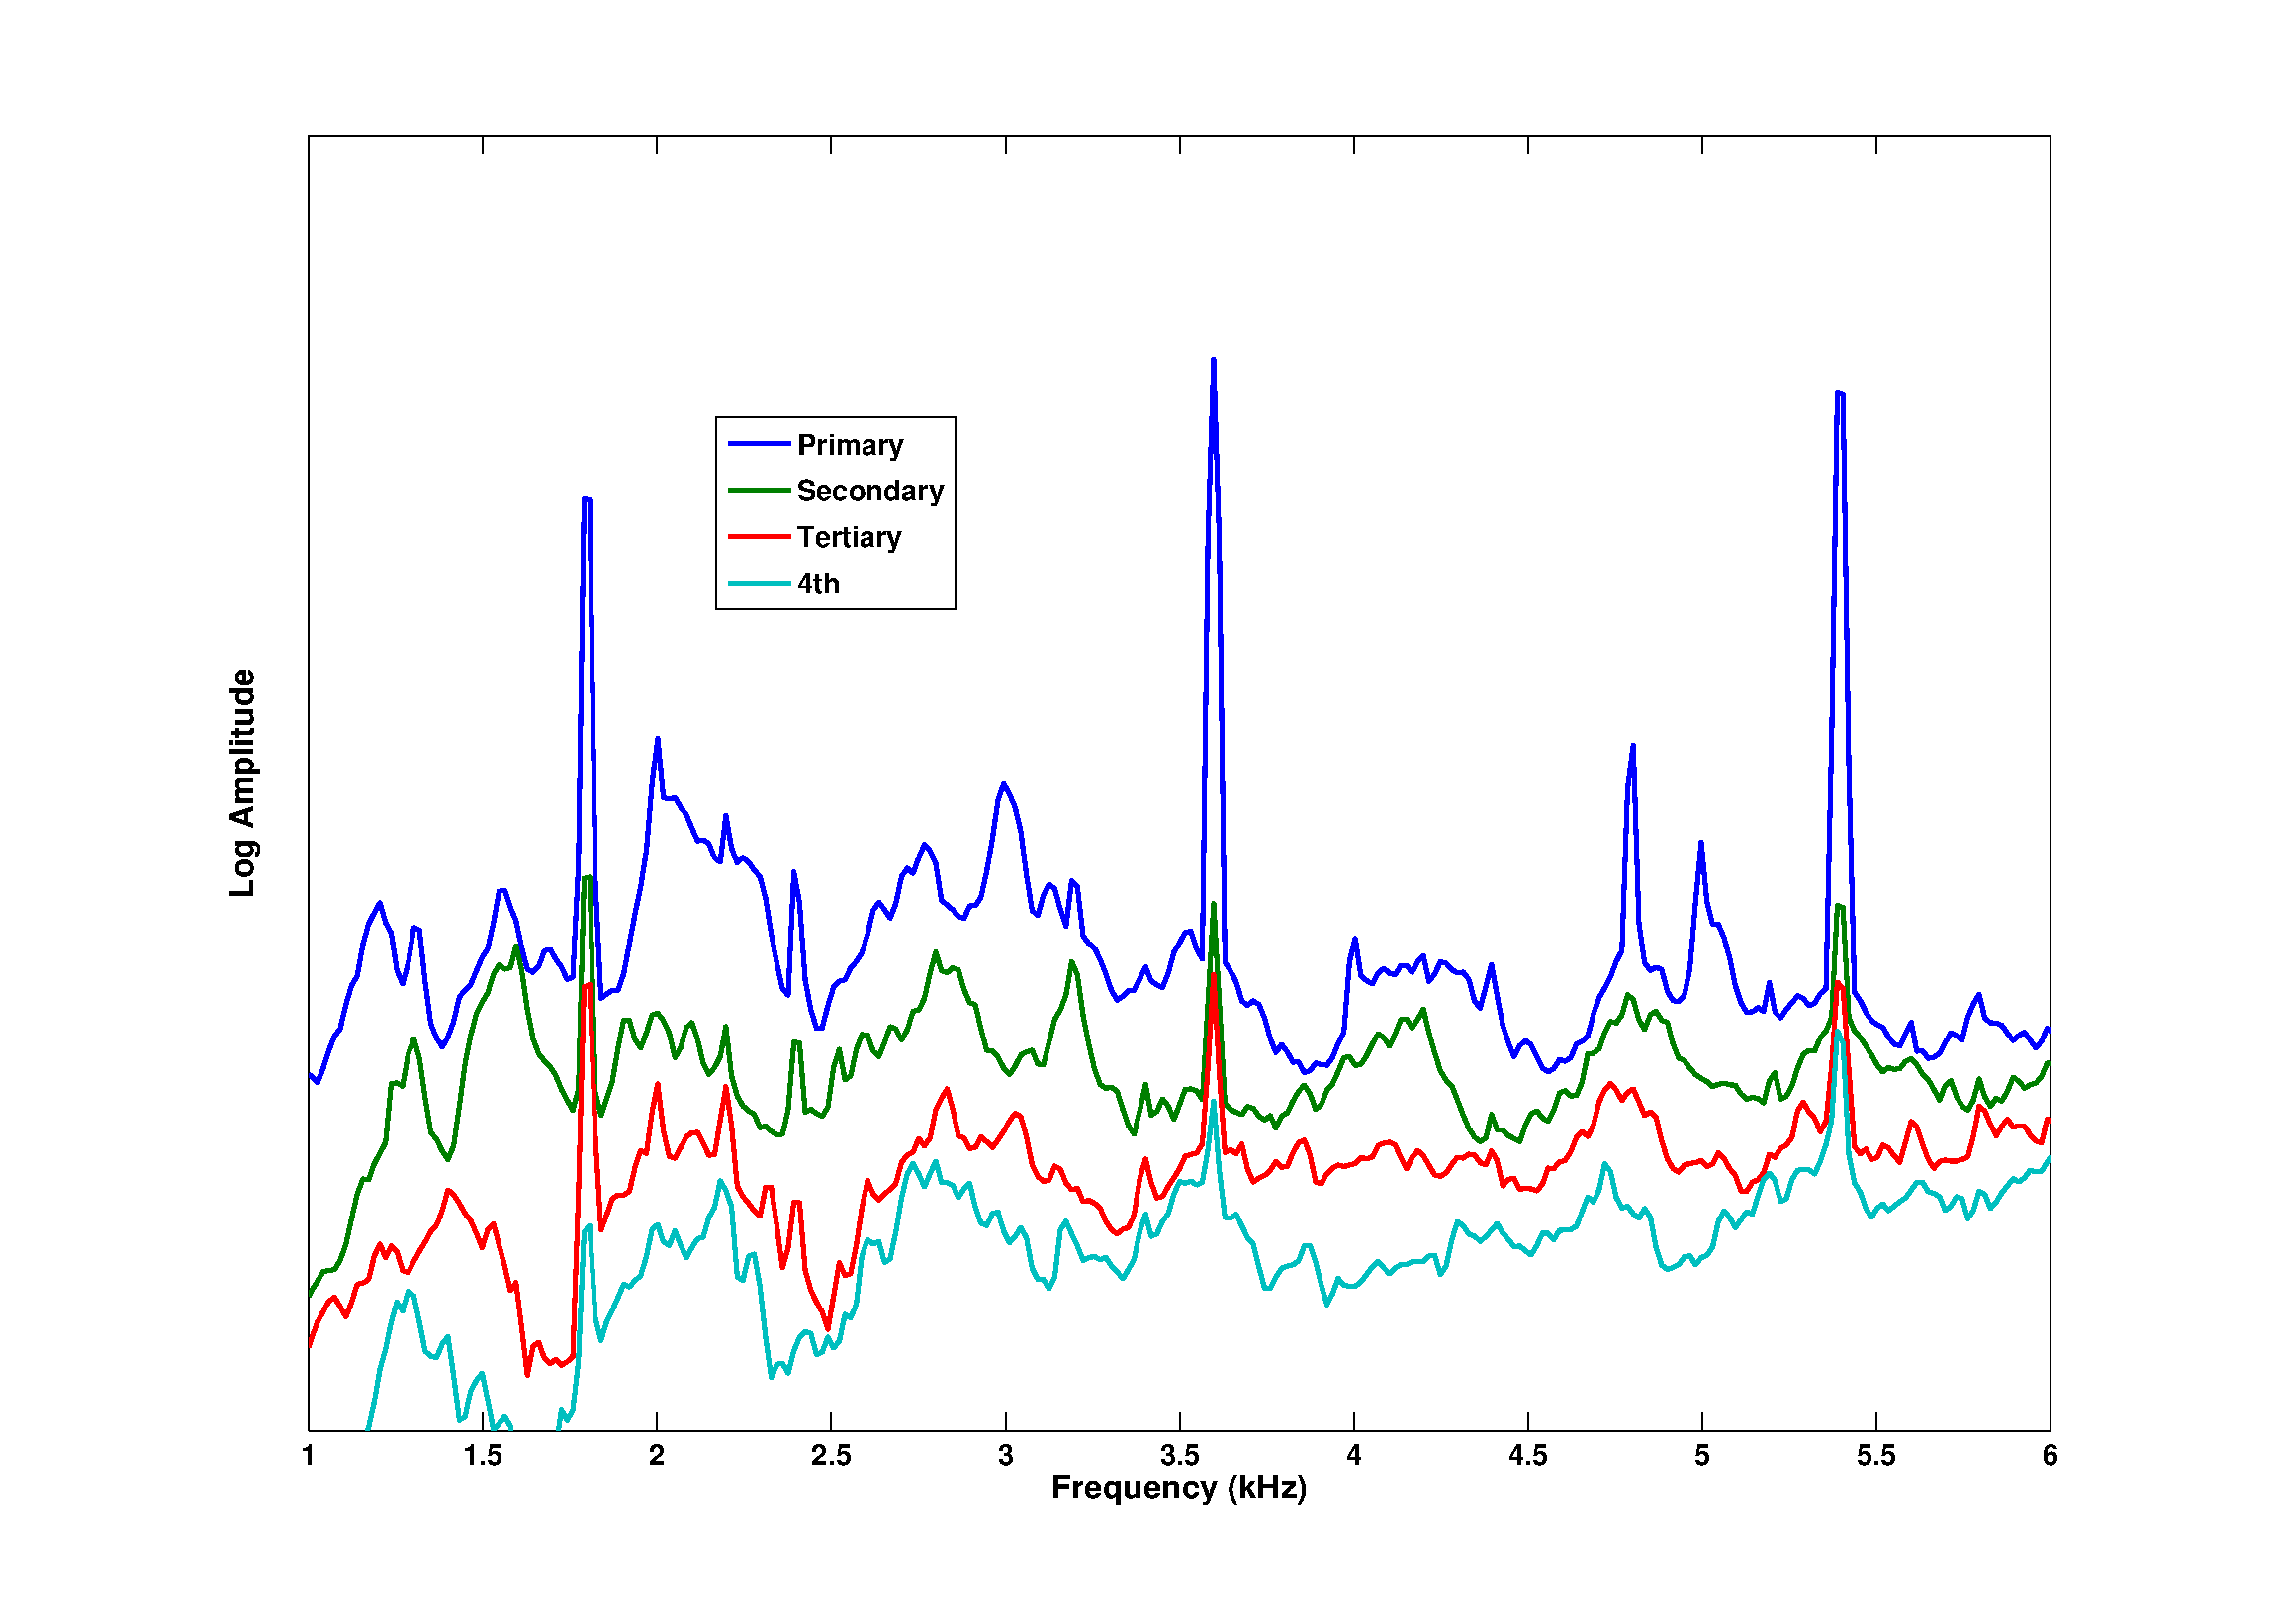
\includegraphics[width=10cm,trim=0 25 0 25]{evals}
  \end{figure}
}

\frame{\frametitle{Wold Decomposition of Center Traversing Microphone} 
  Time histories of
  sinusoids and broadband noise as function of traverse distance.  The exhaust is to the
  right in the figure. \qquad \qquad \raisebox{-2ex} {\Huge $\Longrightarrow$}
  \only<1>{
    \begin{figure}
      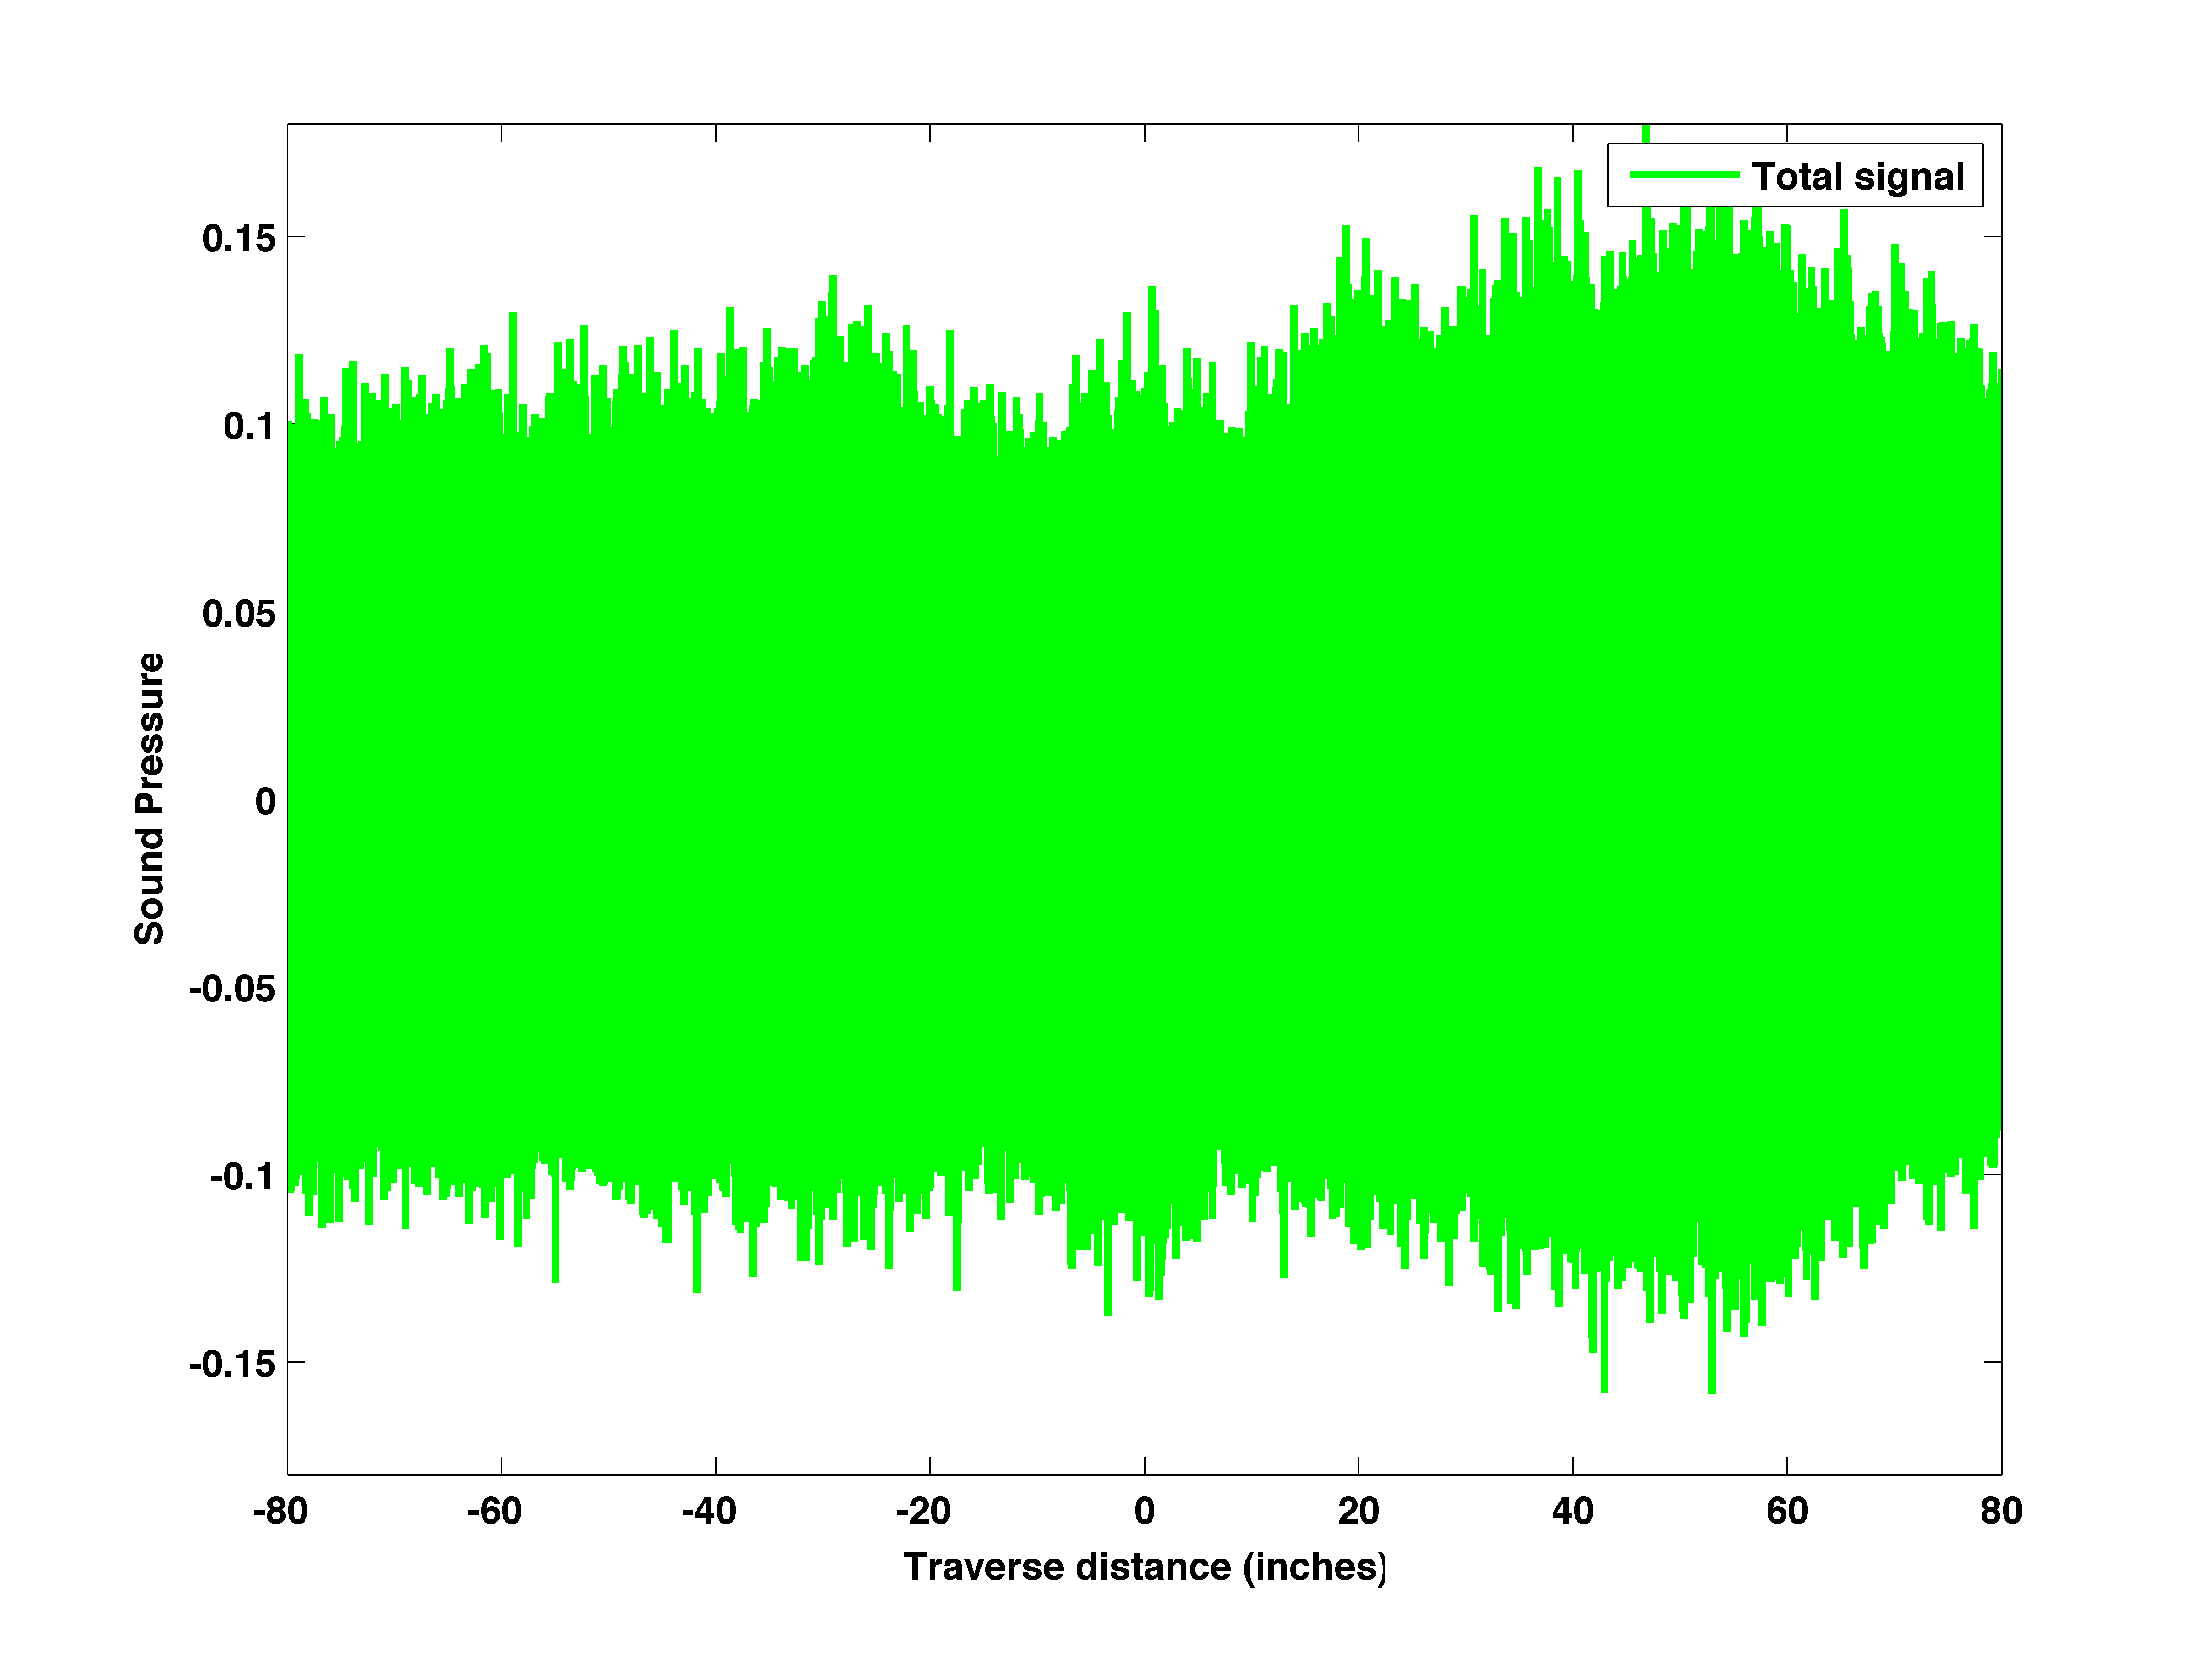
\includegraphics[width=10cm,height=7cm,trim=0 0 0 15]{pc1s2decomp_total_600}
    \end{figure}} \only<2>{
    \begin{figure}
      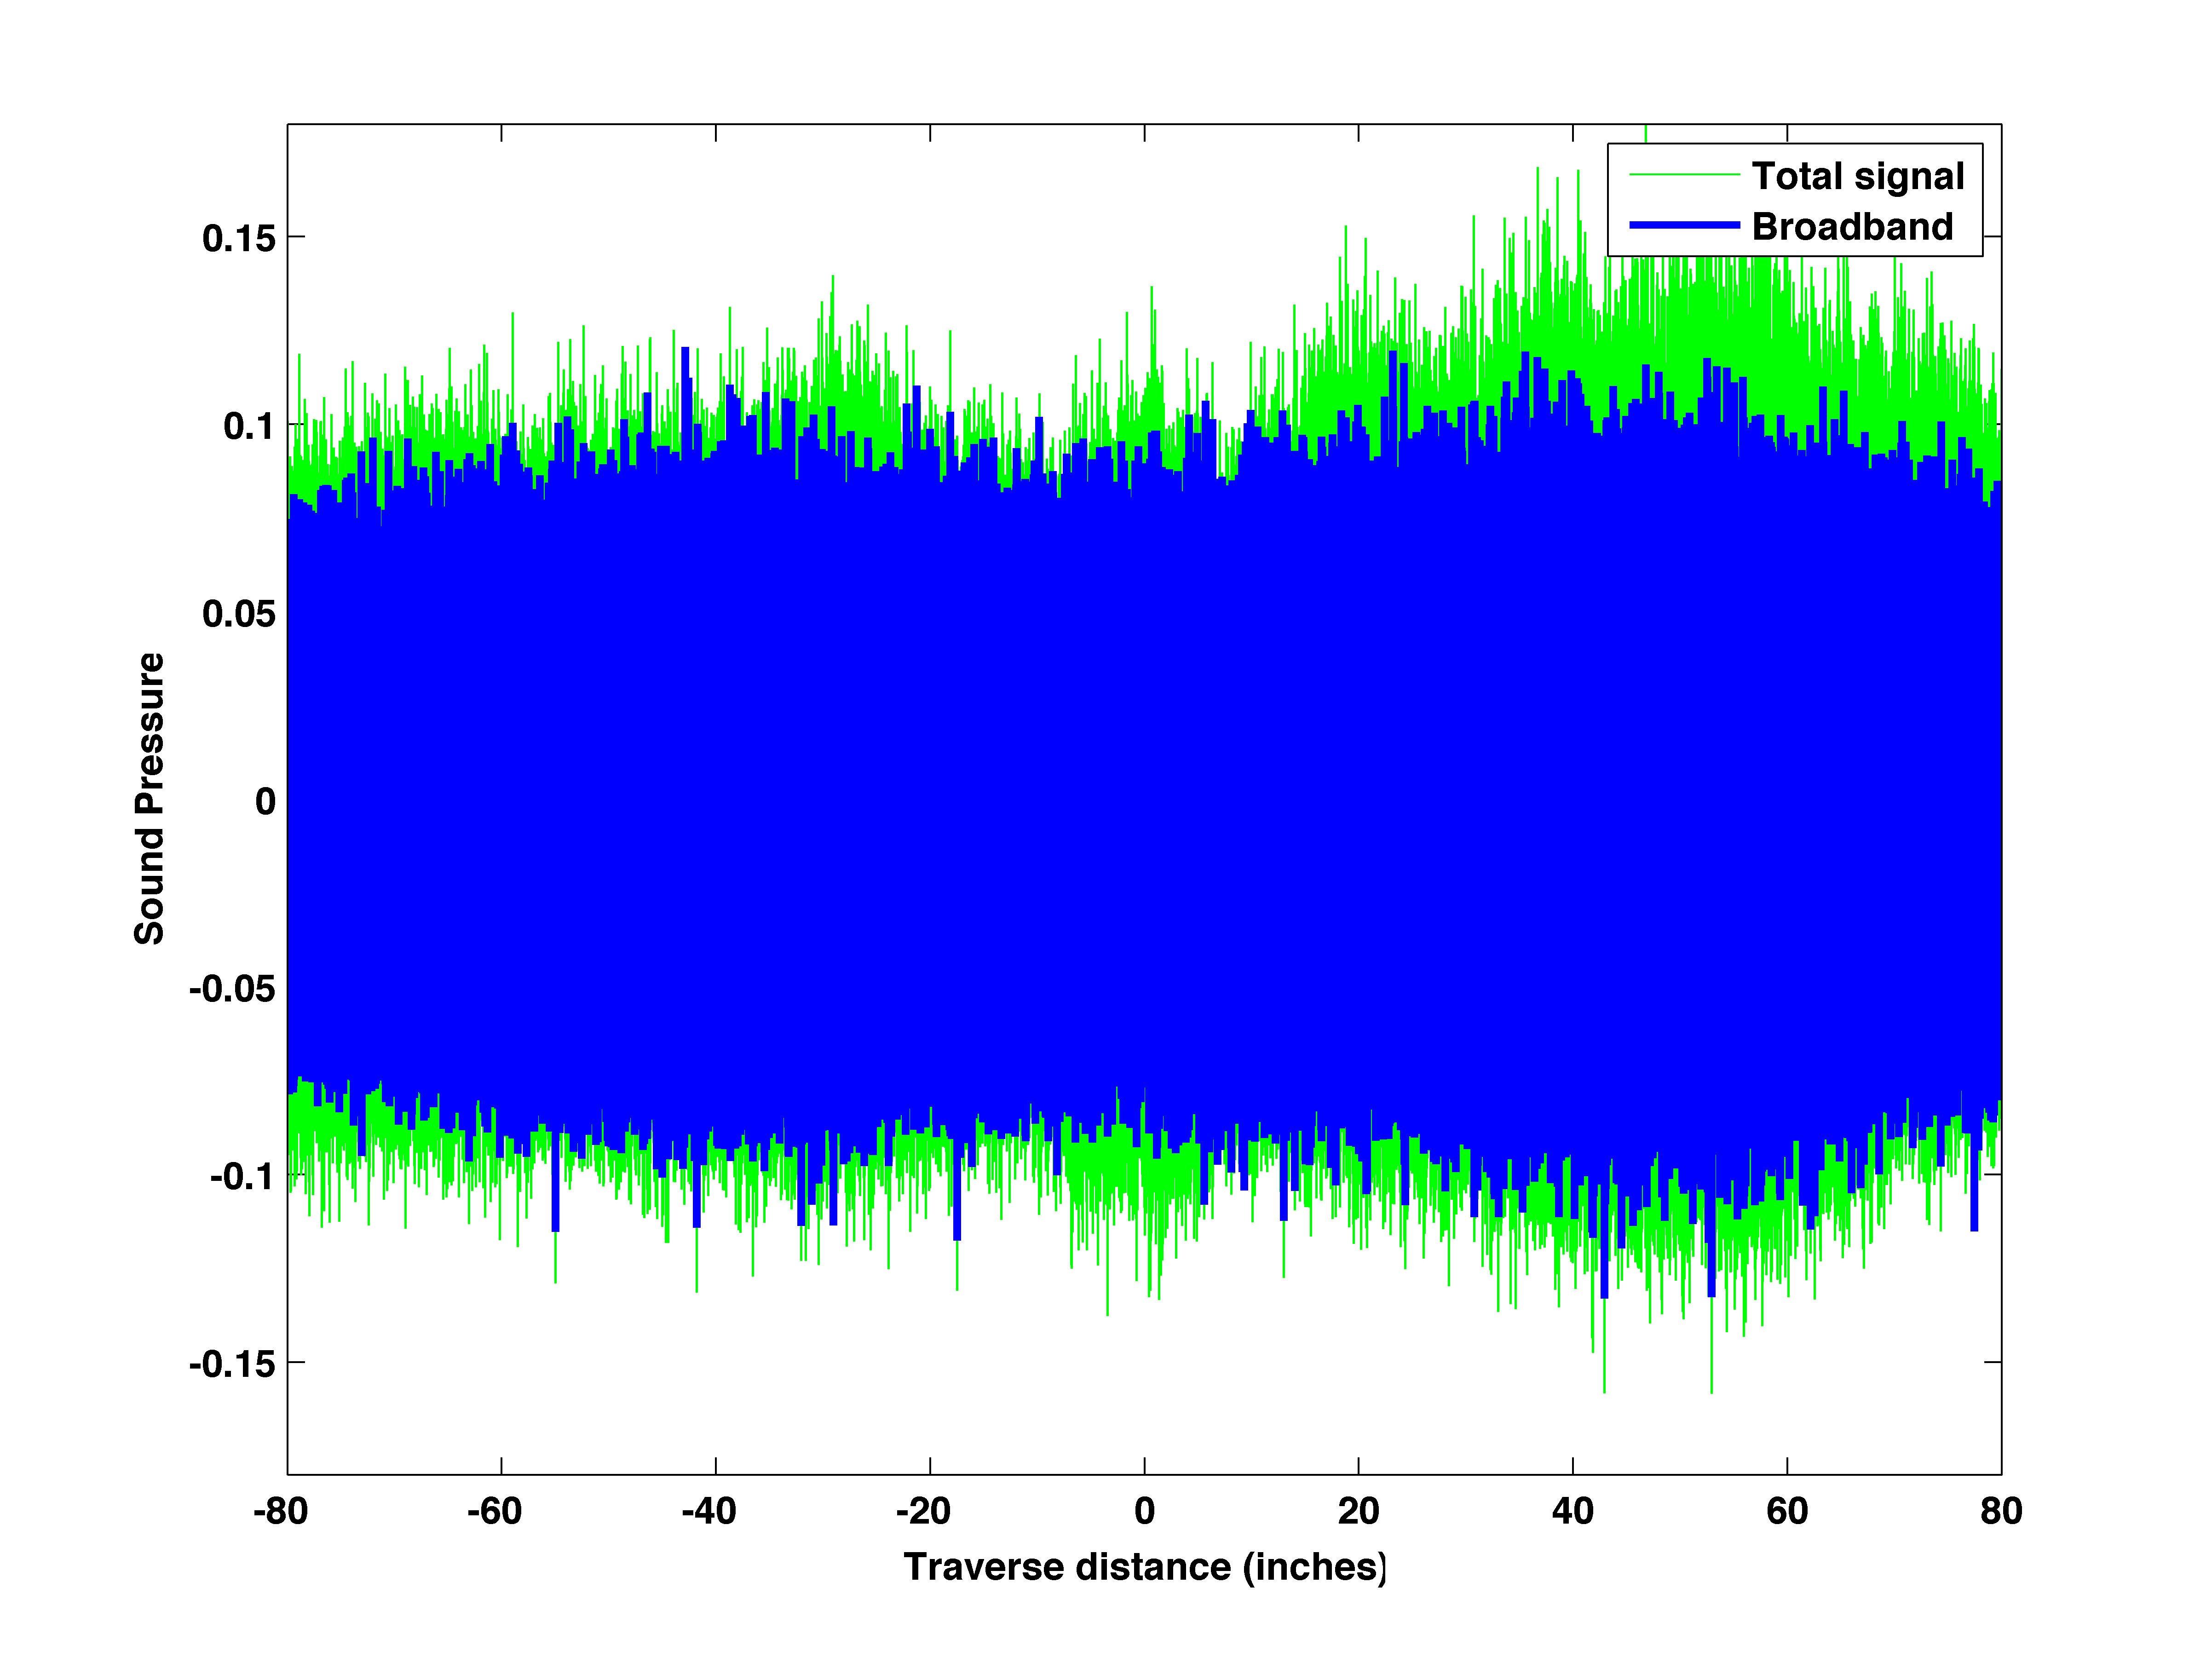
\includegraphics[width=10cm,height=7cm,trim=0 0 0 15]{pc1s2decomp_broad_600}
    \end{figure}} \only<3->{
    \begin{figure}
      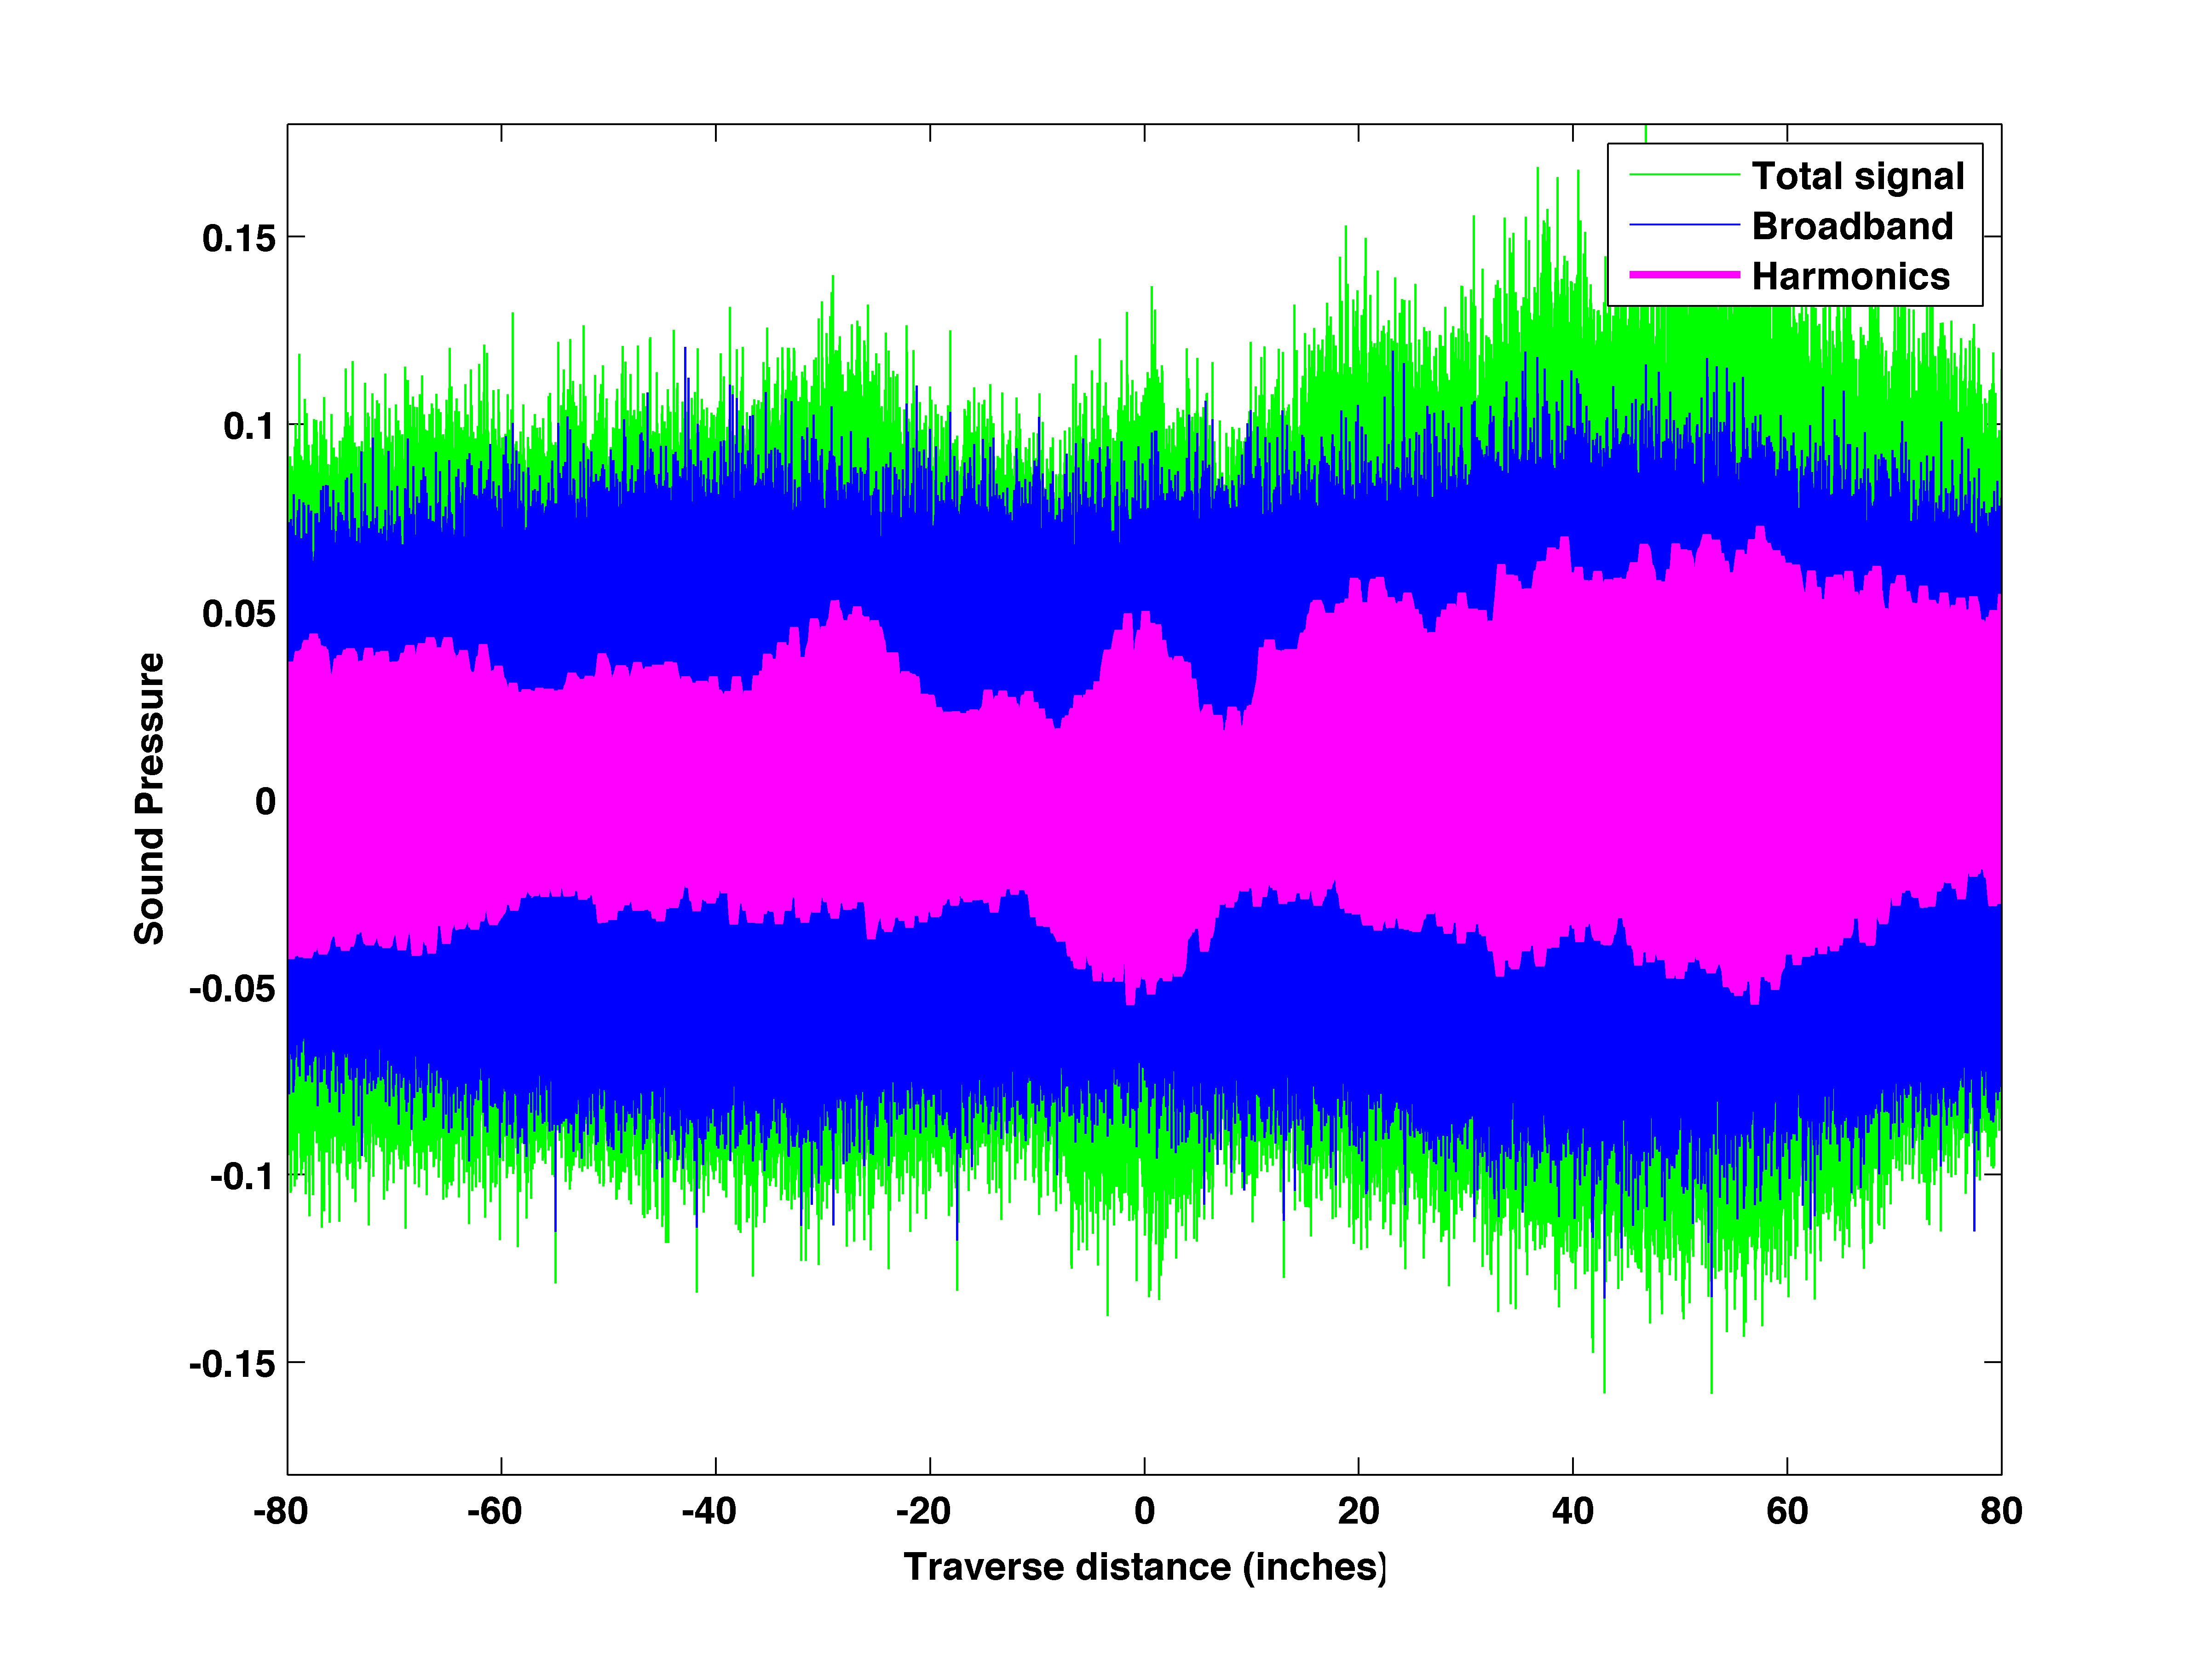
\includegraphics[width=10cm,height=7cm,trim=0 0 0 15]{pc1s2decomp_harm_600}
    \end{figure}} }

\frame{\frametitle{Real Part of Bladepass 2 at Center Traversing Microphone}
  \textbf{\color{blue}{Continuous scan}} compared with \textbf{\color{red}{Fixed index
      (start--stop) with 3\,inch spacing}}. Note spatial aliasing; acoustic wavelength is
  3.7\,inches at 3.6\,kHz.  The exhaust is to the right in the figure. 
  \qquad \qquad \raisebox{-2ex} {\Huge $\Longrightarrow$}
  \begin{figure}
    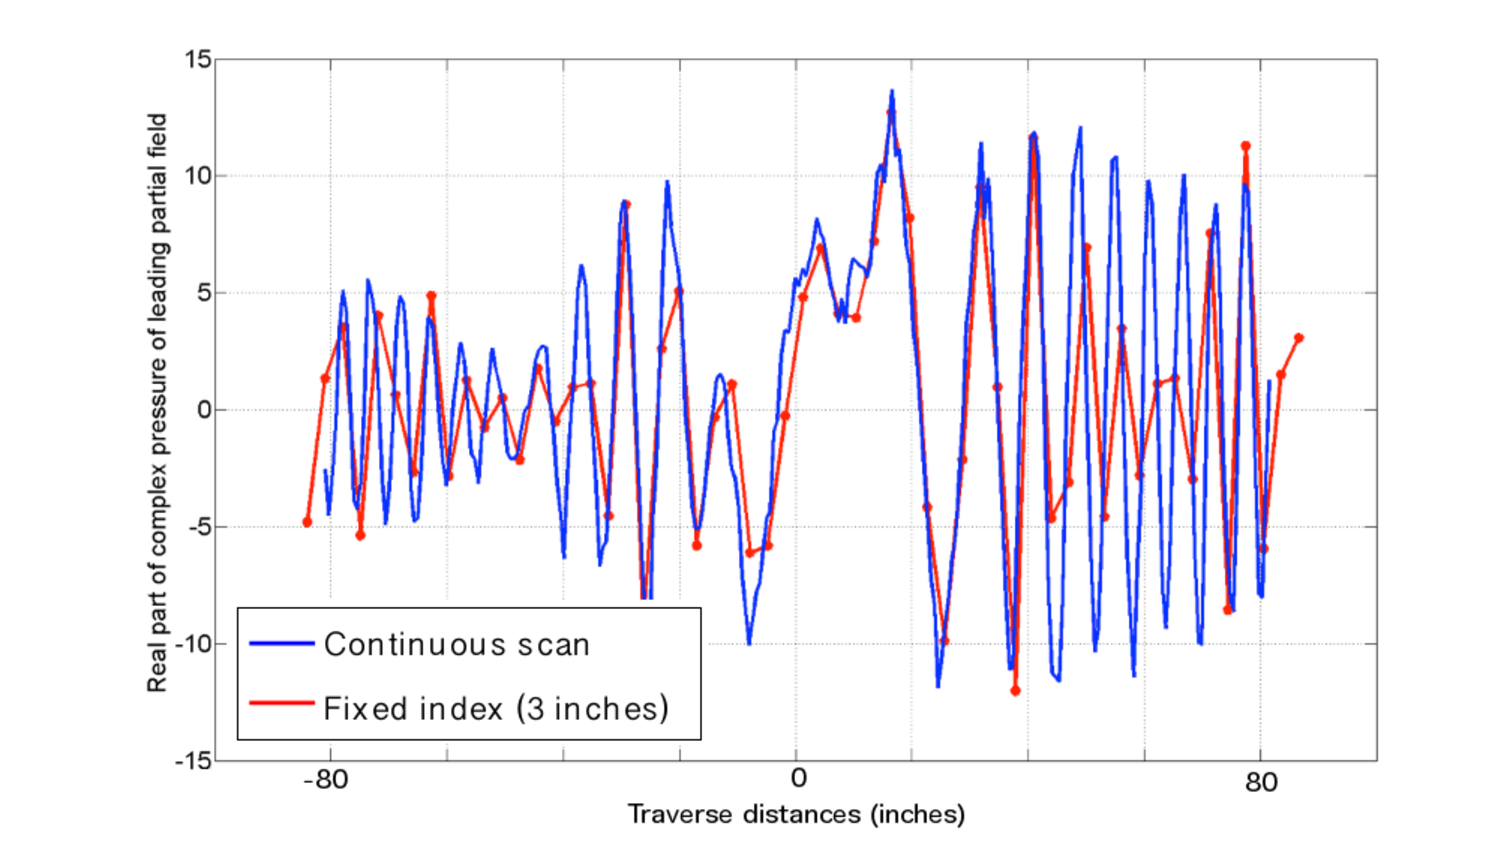
\includegraphics[width=10cm,height=6.5cm,trim=0 0 0 15]{BP2Linescan}
  \end{figure}
}

\frame{\frametitle{Fourier Acoustics Reconstruction of BP 2 Sound Field}
  \begin{columns}[T]
    \column{0.6\paperwidth}
    \begin{figure}
      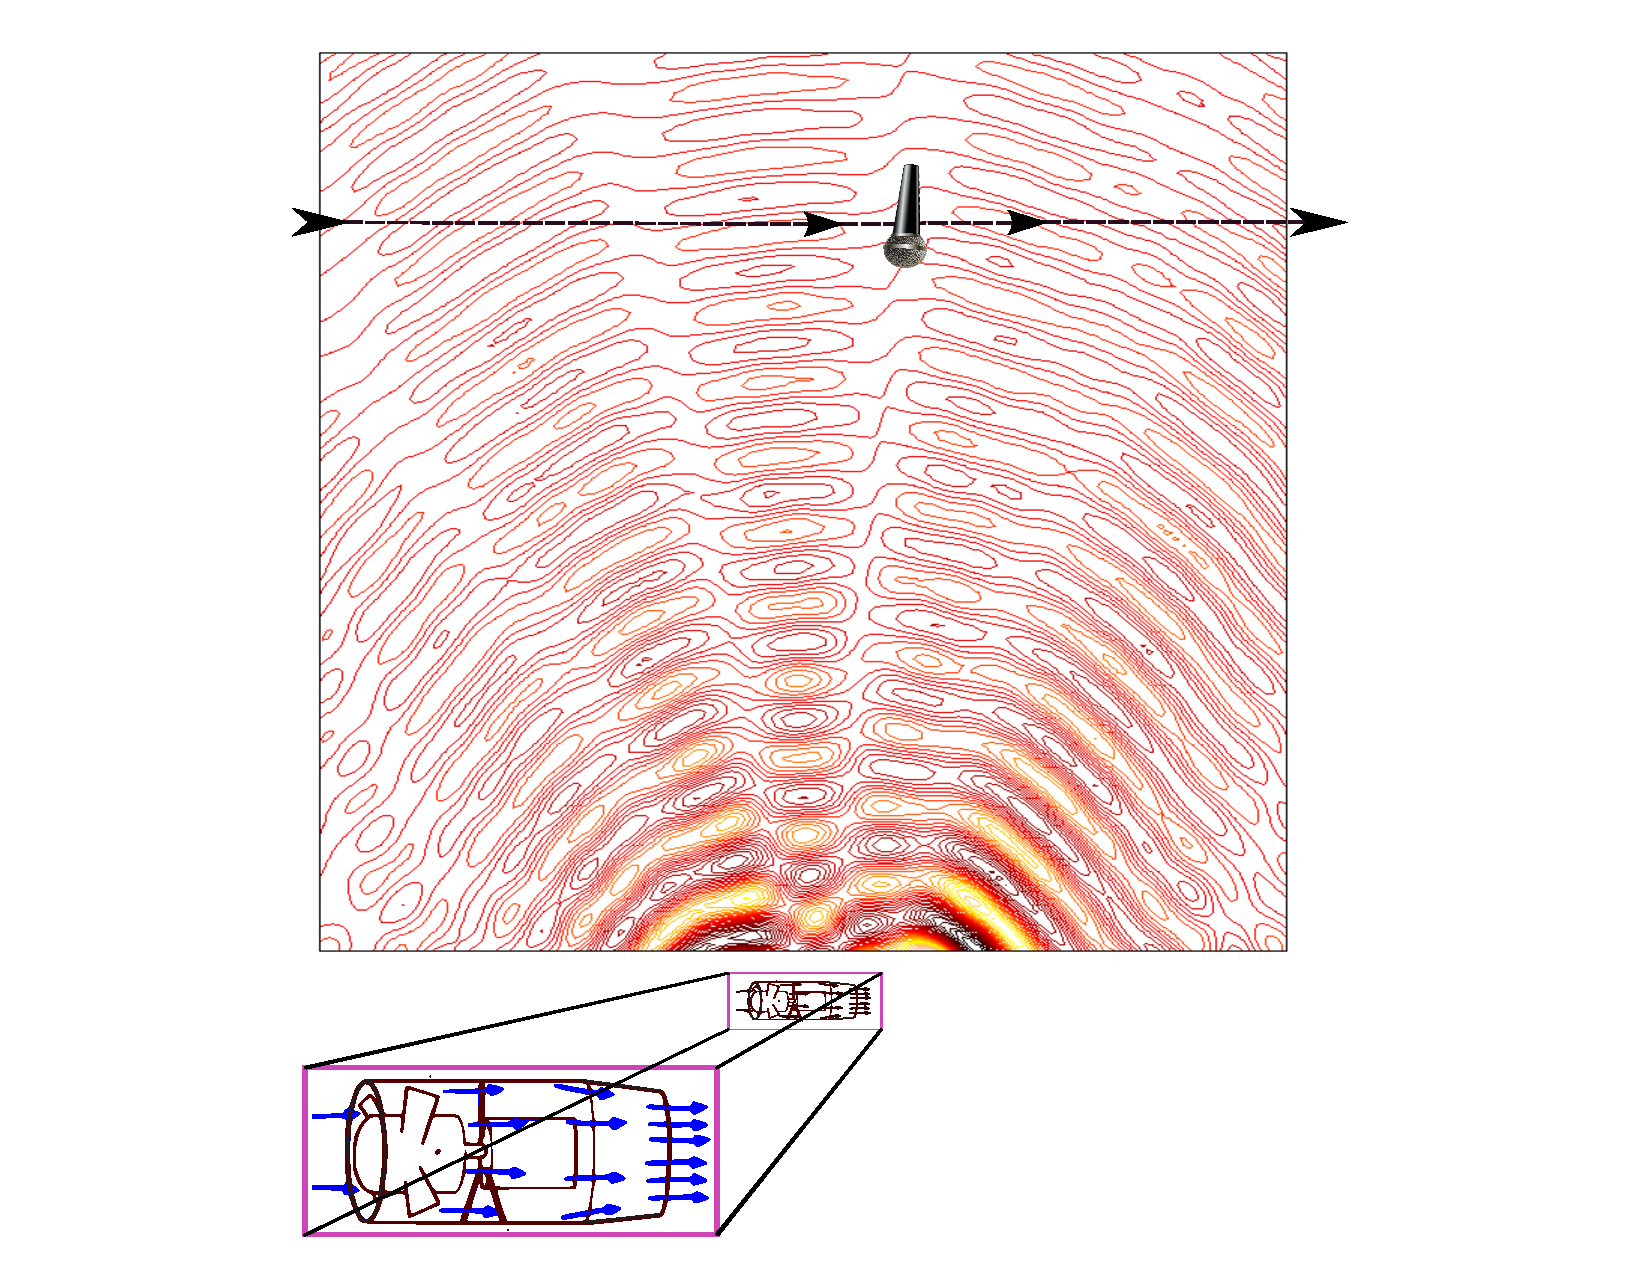
\includegraphics[width=9cm,trim=40 0 0 75]{FanWorkSheet.pdf}
    \end{figure}
    \column{0.4\textwidth} \alert<1>{Continuous scan eliminates spatial aliasing at higher
      frequencies, allowing for the
      techniques of \emph{acoustic holography} to be used. \\
      Axisymmetry is assumed.} \\
    \uncover<2>{\alert<2>{Resolution at source limited by acoustic wavelength;
        \emph{evanescent} waves have died before they reach the microphone.}}
  \end{columns}
}

\frame{\frametitle{Fourier Acoustics 1200\,Hz Broadband Sound Fields}
  \begin{columns}[T]
    \column{0.5\textwidth}
    \vspace{-0.7em}
   \center{Primary $6^{th}$ octave field\\ \alert<1>{Antisymmetric}}
    \begin{figure}
      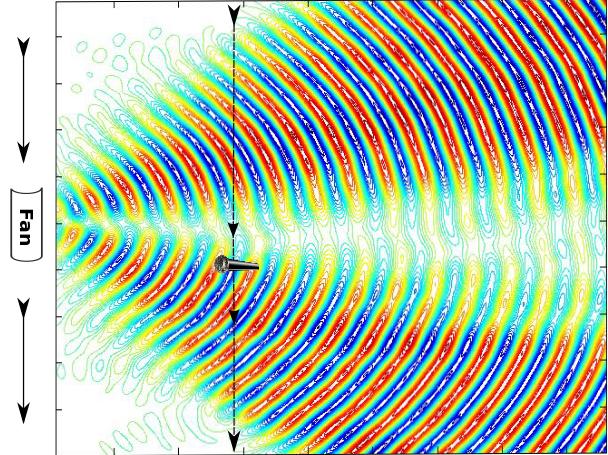
\includegraphics[width=6cm,height=5cm,angle=90]{1200F1}
    \end{figure}
    \column{0.5\textwidth}
    \vspace{-0.7em}
    \center{Secondary $6^{th}$ octave field\\ \alert<2>{Symmetric}}
    \begin{figure}
      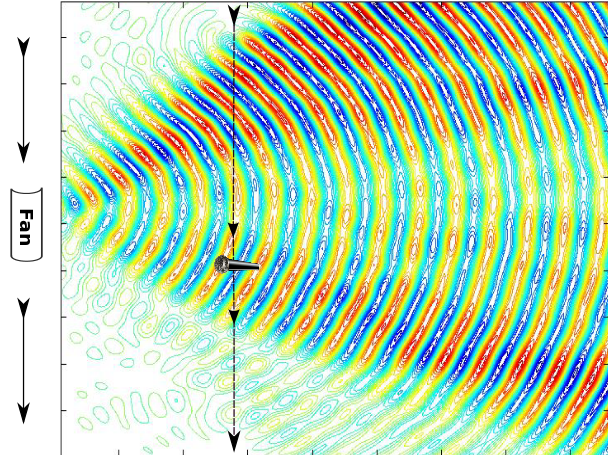
\includegraphics[width=6cm,height=5cm,angle=90]{1200F2}
    \end{figure}
  \end{columns}
  \center{Amplitudes scaled for graphics presentation}
}

\section{Dual Open Rotor in NASA Glenn 9x15 Wind Tunnel}
\frame{\frametitle{Dual Open Rotor in NASA Glenn 9x15 Wind Tunnel} 
  Two counter-rotating
  rotors\uncover<2->{, \color{red}{loosely coupled through control system}}
  \begin{columns}
    \column{0.45\textwidth}<1->
    \begin{figure}
      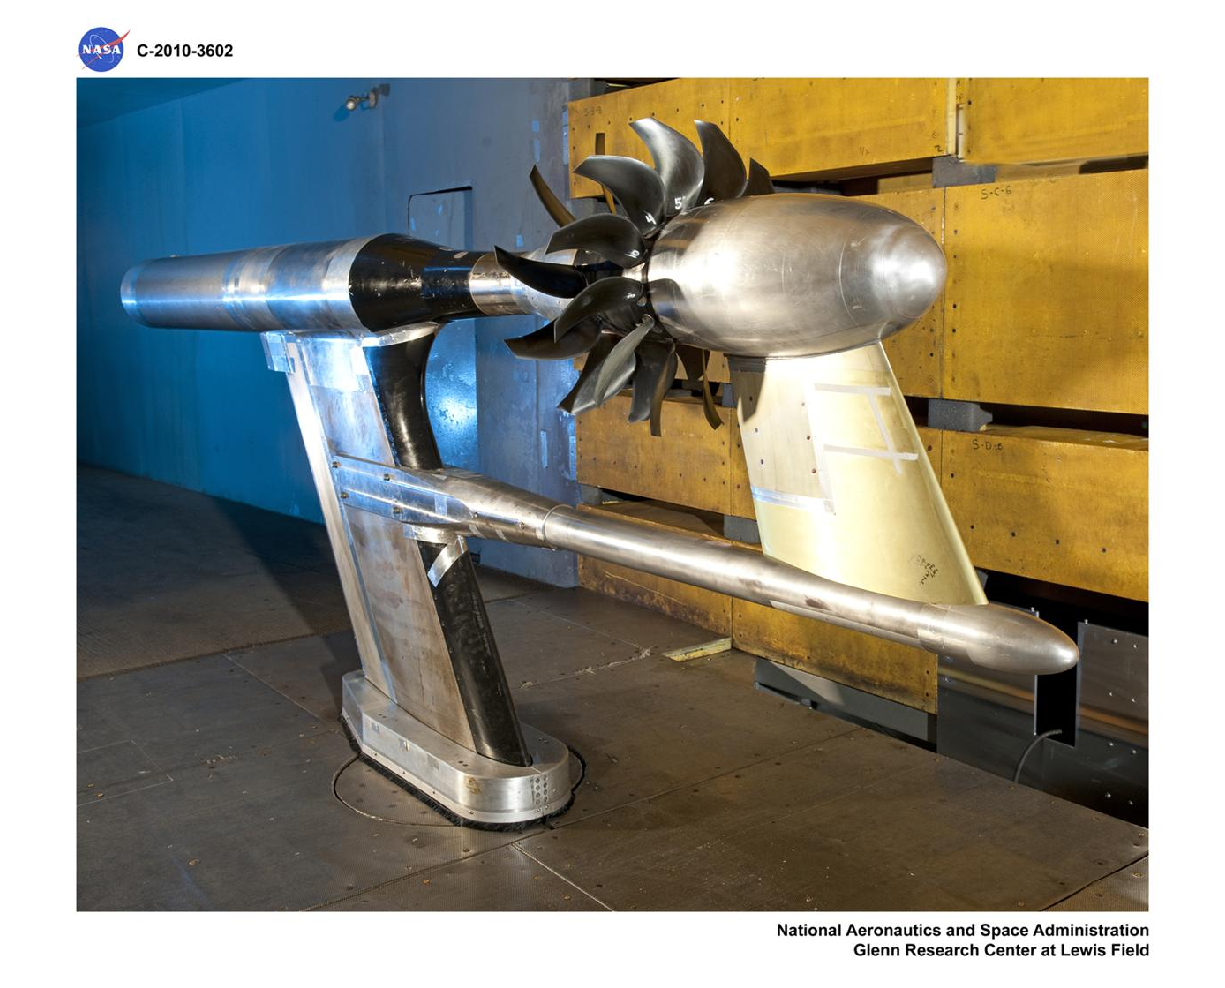
\includegraphics[height=5cm]{2010_03602_150_Small}
    \end{figure}
    \center{\color{black}{Back to the future\\Hardware anno 1988}} 
    \column{0.55\textwidth}<2->
    \vspace{1cm}
    \begin{figure}
      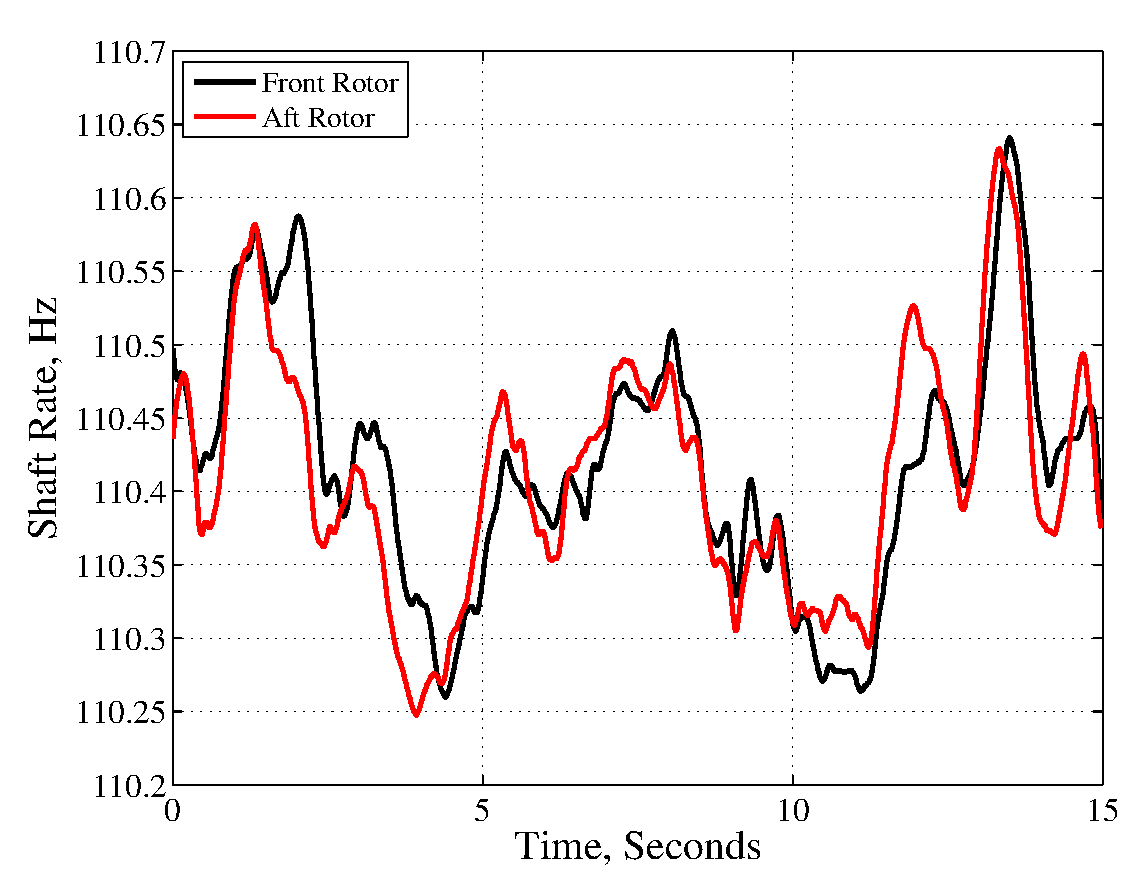
\includegraphics[width=5cm,height=4cm]{RPM_Example_472_8}
    \end{figure}
    \center{\alert<2->{Time histories of rotor speeds}}
  \end{columns}
}

\frame{\frametitle{Removing Tones with the Vold-Kalman Filter} \only<1>{ \center{PSD of
      total signal\\Tones and broadband noise}
    \begin{figure}
      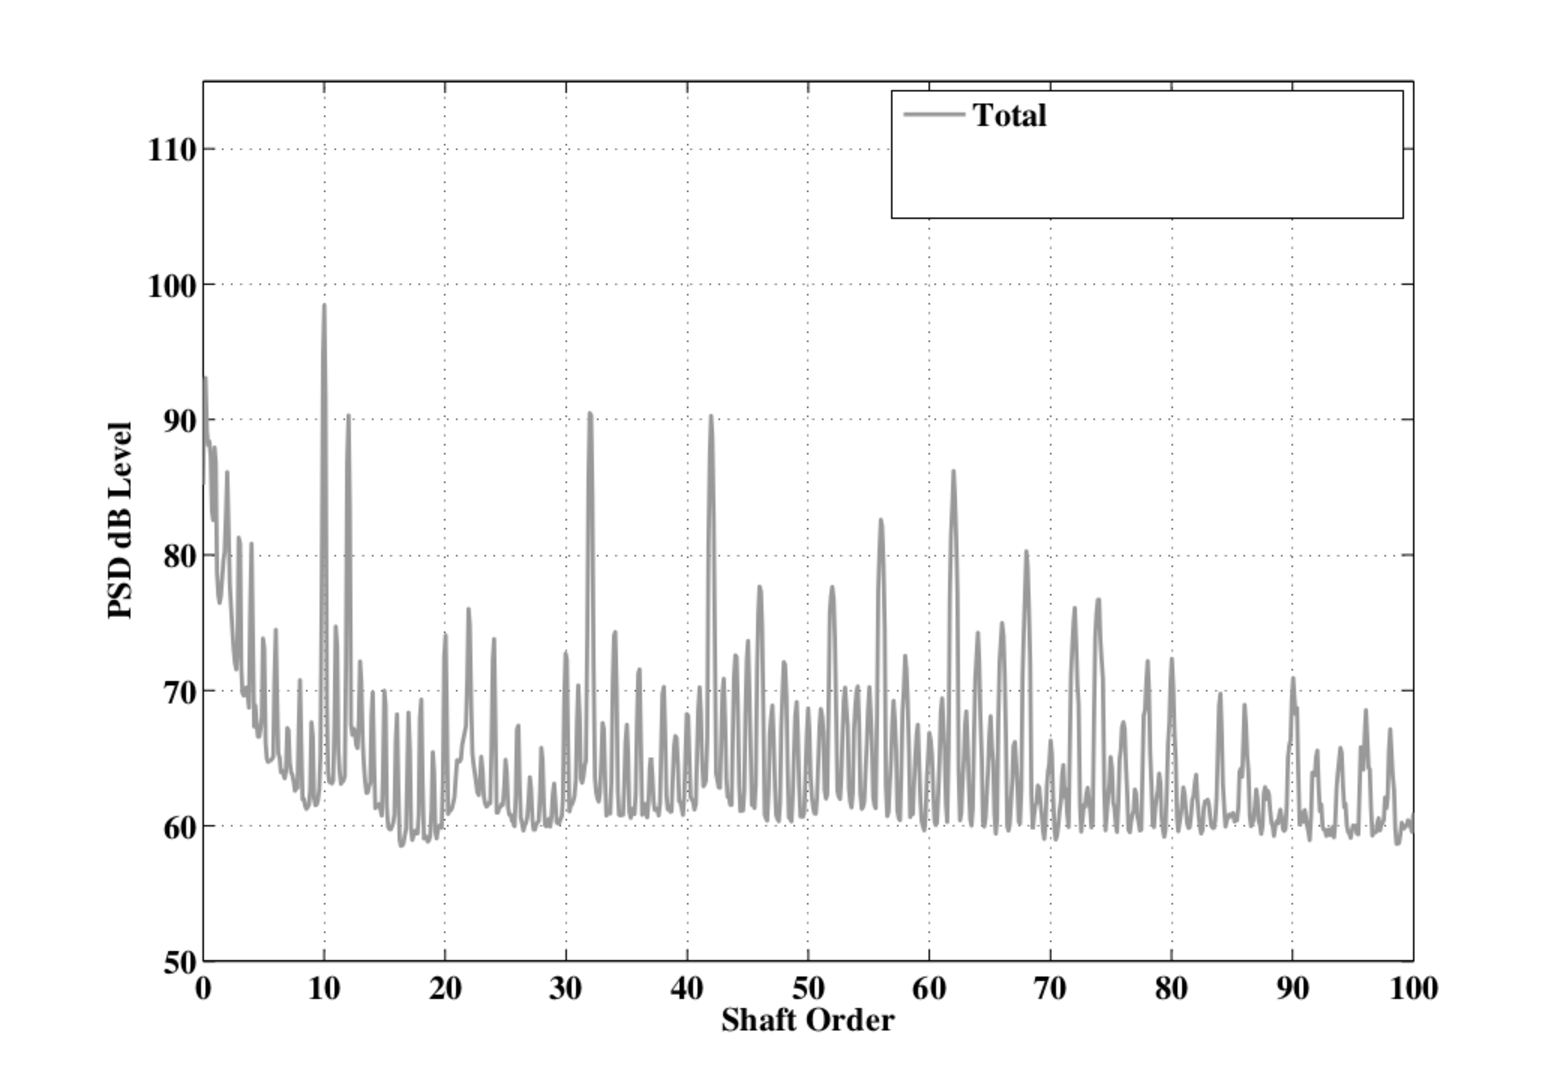
\includegraphics[width=10cm]{RDG_446_VK_Compare_total}
    \end{figure}} \only<2>{ \center{PSD of signal with tones removed
      shaft--by--shaft\\Interaction tones cause trouble}
    \begin{figure}
      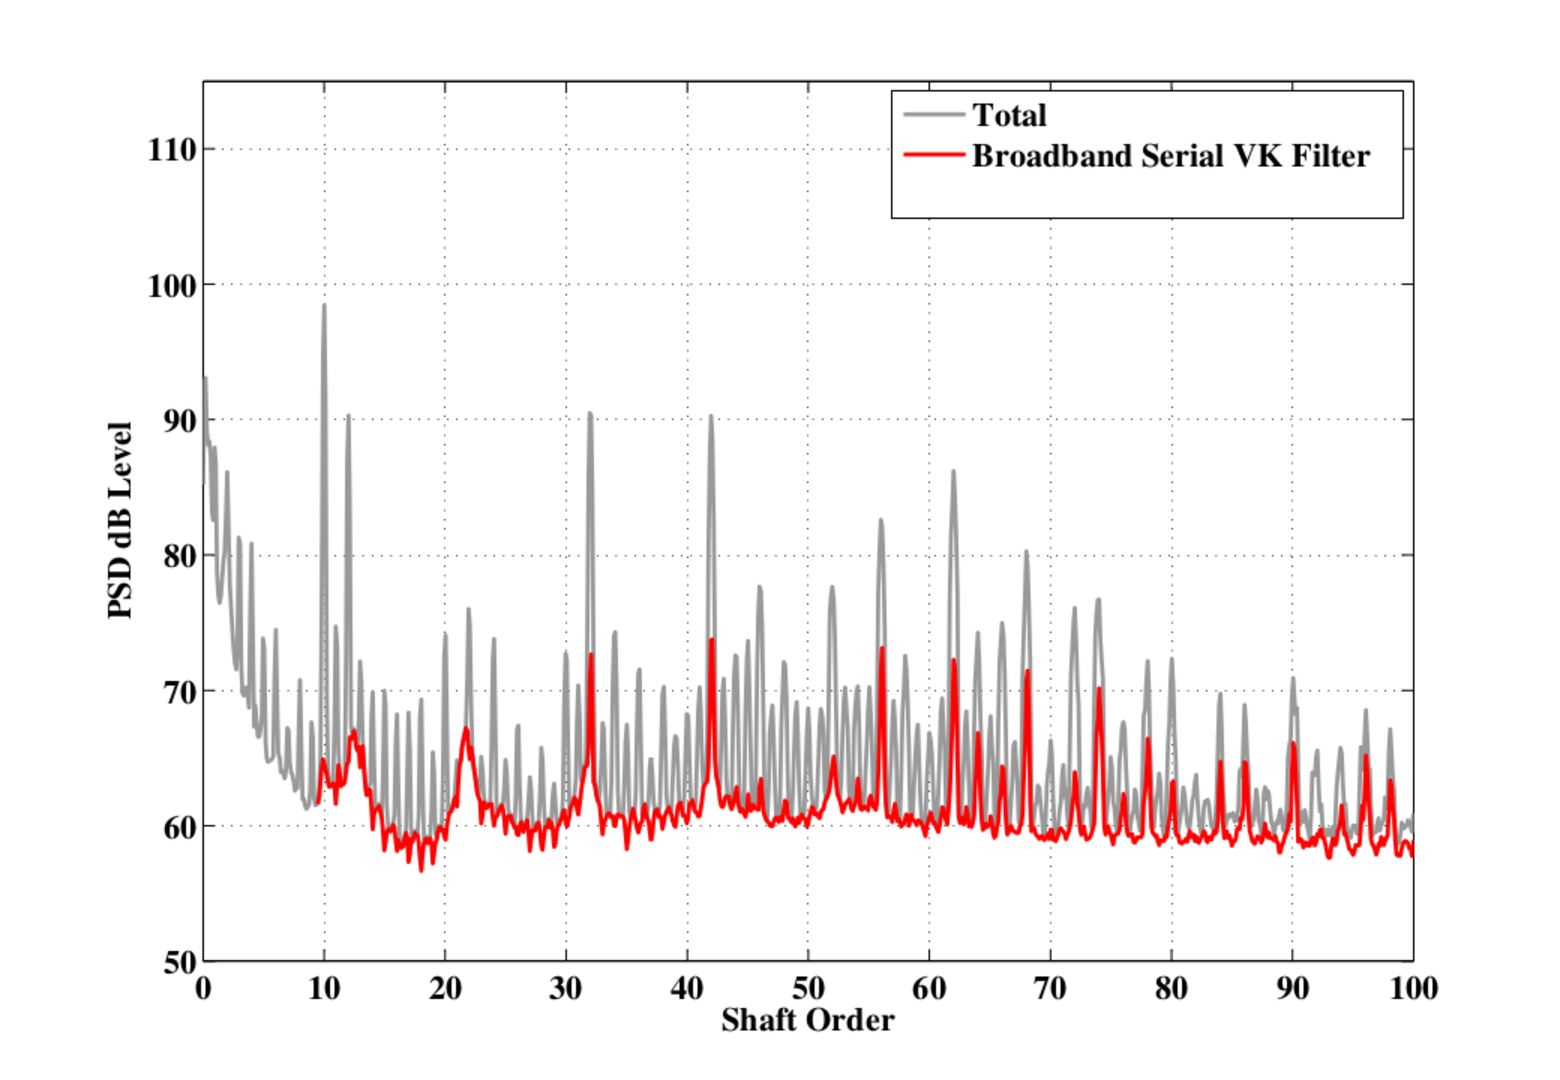
\includegraphics[width=10cm]{RDG_446_VK_Compare_serial}
    \end{figure}} \only<3->{ \center{PSD of signal with tones removed
      simultaneously\\Interaction tones behave}
    \begin{figure}
      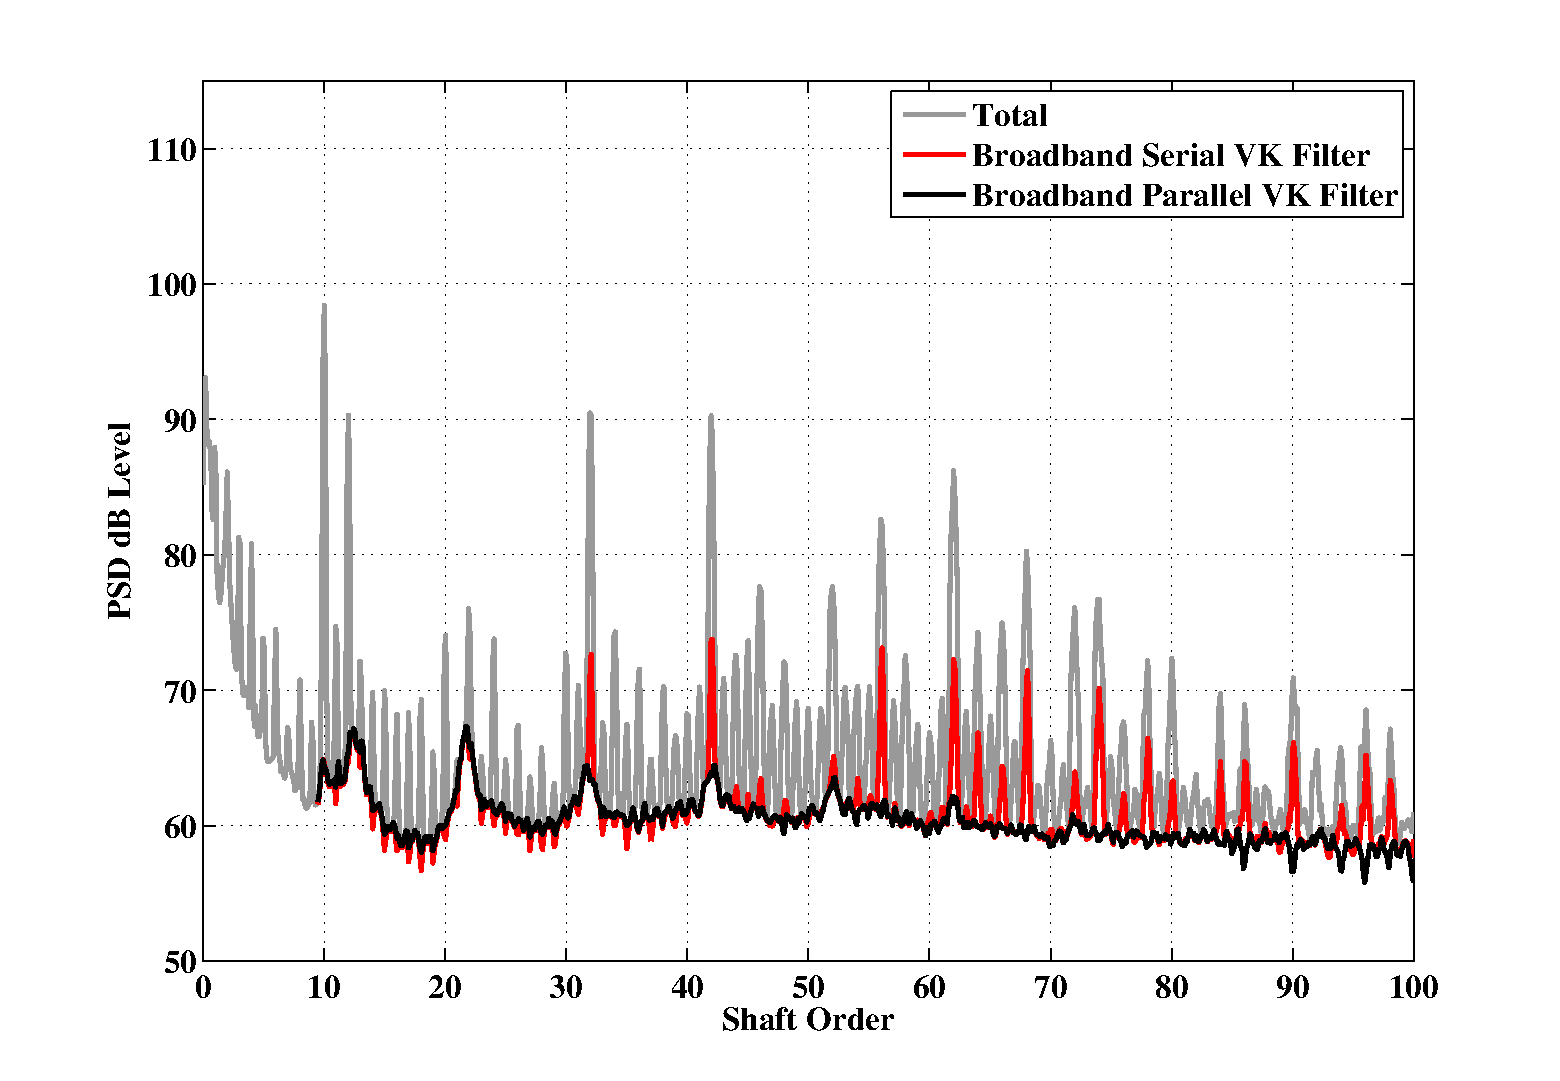
\includegraphics[width=10cm]{RDG_446_VK_Compare_parallel}
    \end{figure}} }

\begin{frame}
\frametitle{Fourier Acoustics Sound Fields --- Tones 40 and 48}
{ Continuous scan over 6.6\,meters, 600 second scan\\
Traversing microphone 1.52\,meters from centerline\\
\raisebox{-1ex} {\Huge $\Longleftarrow$} Mach 0.2 mean flow}
\vspace{-1em}
  \begin{columns}[T]
    \column{0.5\textwidth}
   \center{Order 40 Rear}
    \vspace{-1em}
    \begin{figure}
      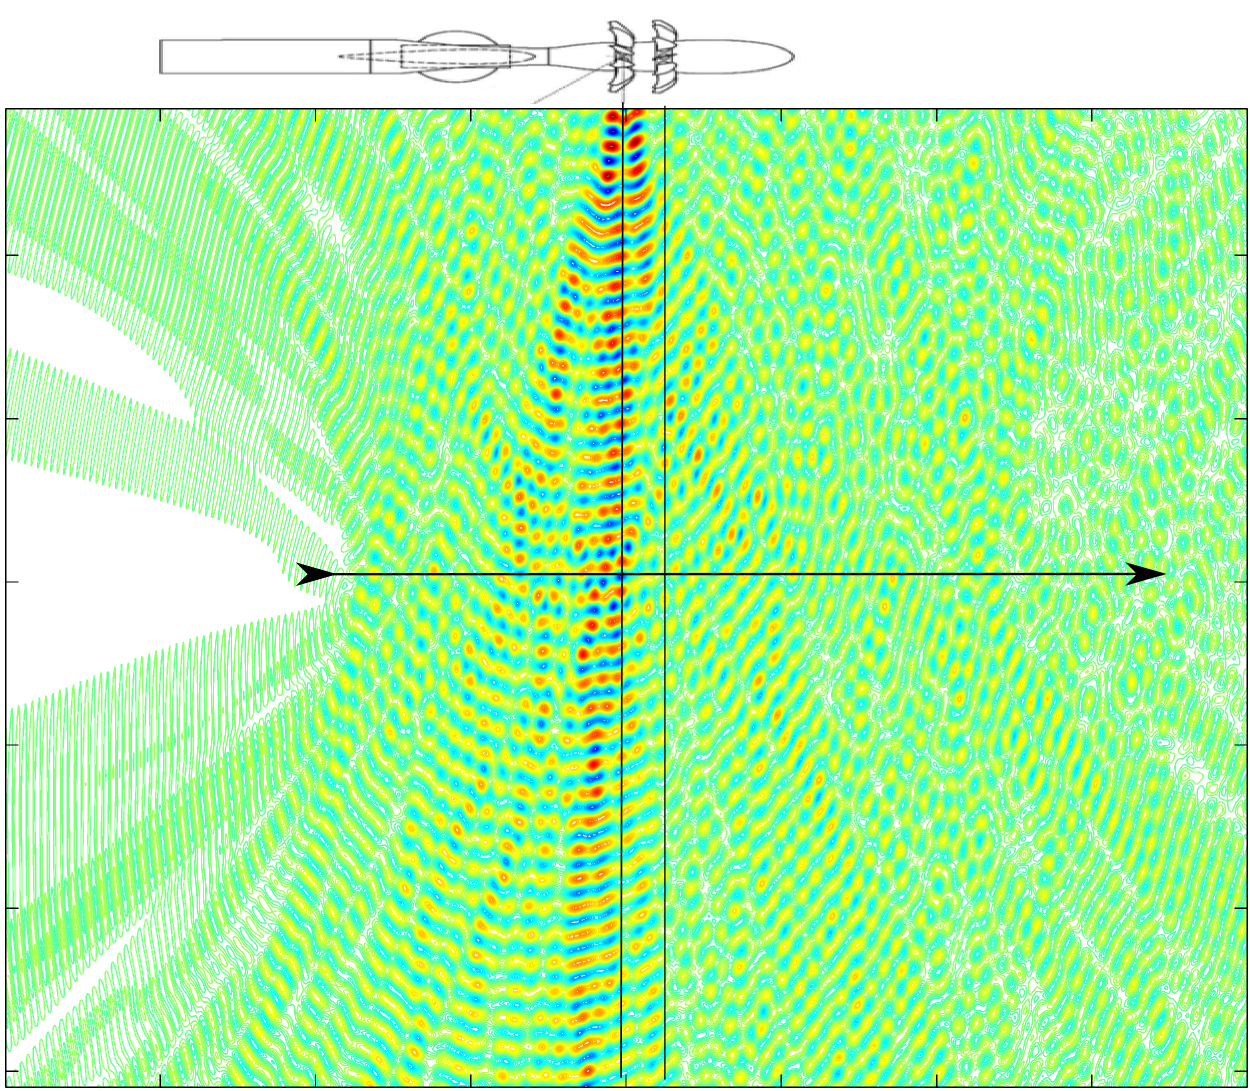
\includegraphics[width=6cm,height=5.5cm]{O40S2H}
    \end{figure}
       \column{0.5\textwidth}
    \center{Order 48 Front}
    \vspace{-1em}
    \begin{figure}
      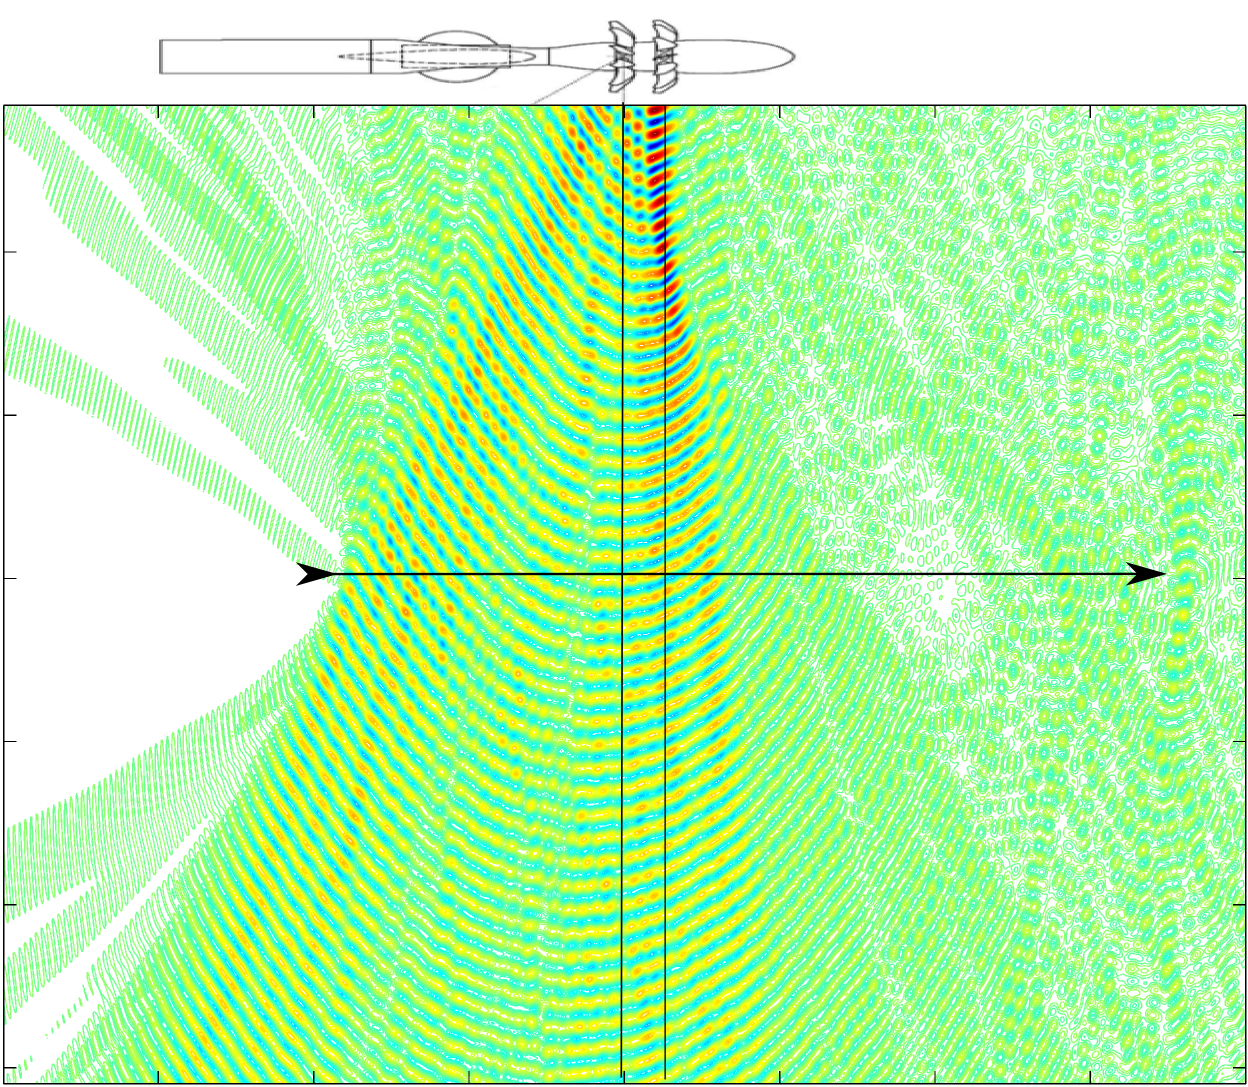
\includegraphics[width=6cm,height=5.5cm]{O48S1H}
    \end{figure}
  \end{columns}
  \center{Amplitudes scaled for graphics presentation}
\end{frame}

\frame{\frametitle{Fourier Acoustics Sound Fields --- Tones 10 and 12}
{Continuous scan over 6.6\,meters, 600 second scan\\
Traversing microphone 1.52\,meters from centerline\\
\raisebox{-1ex} {\Huge $\Longleftarrow$} Mach 0.2 mean flow}
\vspace{-1em}
  \begin{columns}[T]
    \column{0.5\textwidth}
   \center{Order 10 --- Aft Rotor}
    \vspace{-1em}
    \begin{figure}
      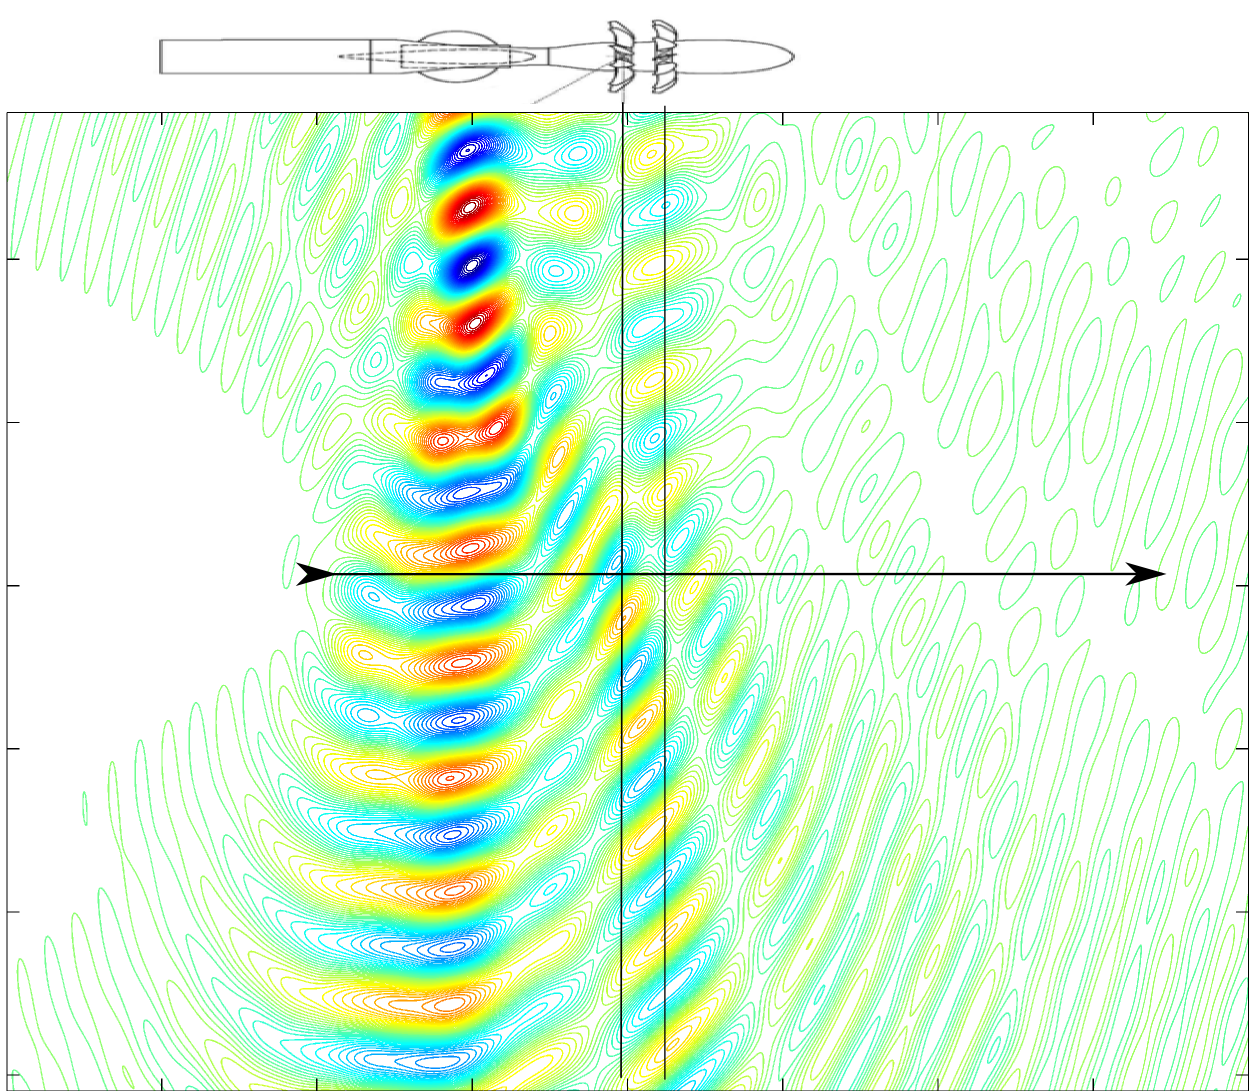
\includegraphics[width=6cm,height=5.5cm]{O10S2H}
    \end{figure}
    \column{0.5\textwidth}
    \center{Order 12 --- Front Rotor}
    \vspace{-1em}
 \begin{figure}
      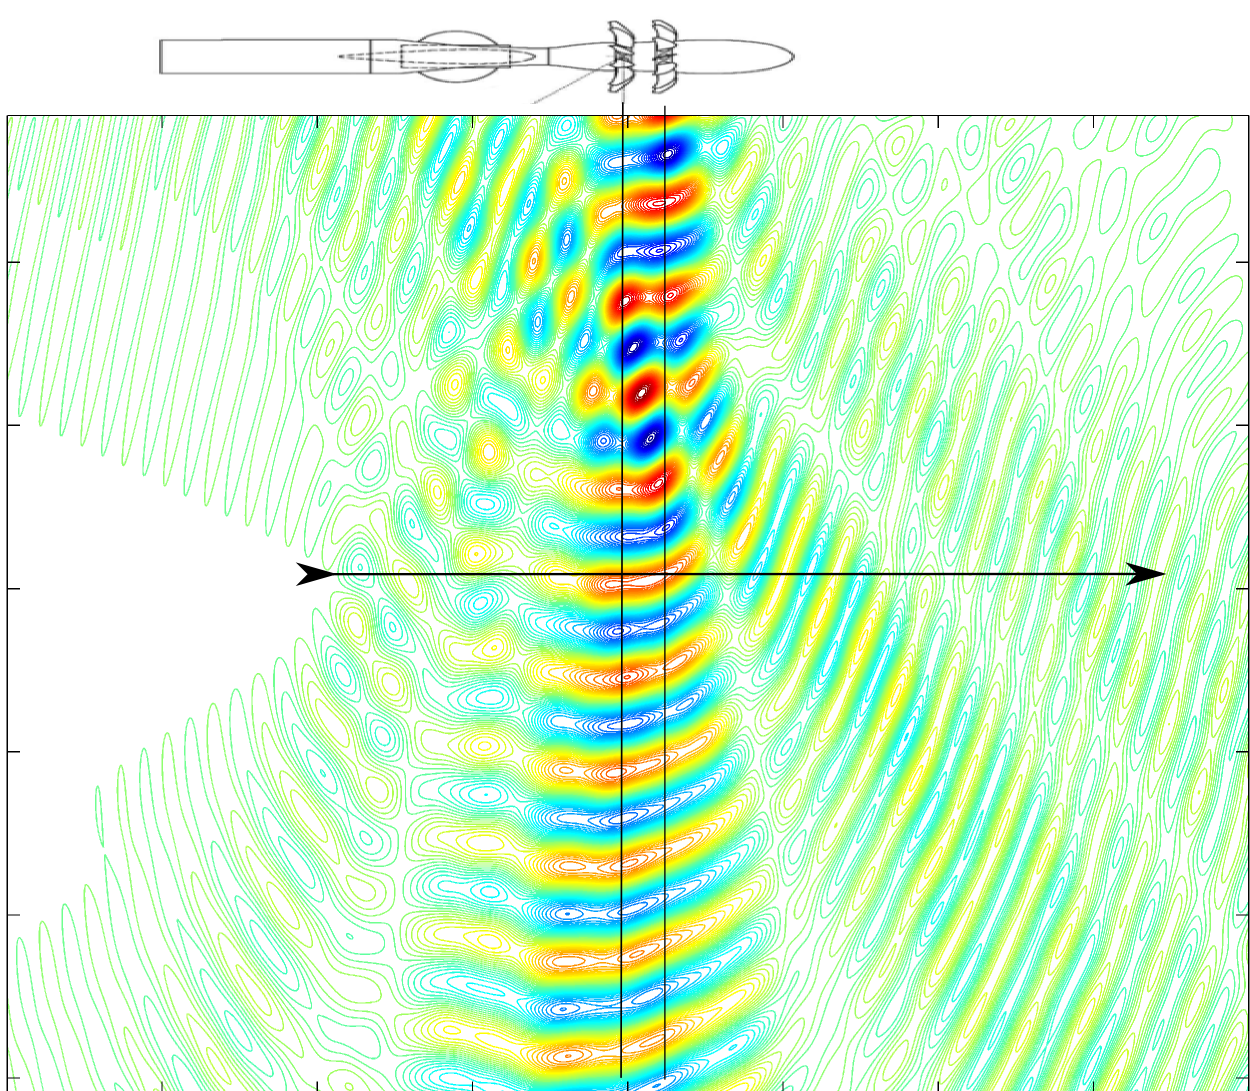
\includegraphics[width=6cm,height=5.5cm]{O12S1H}
    \end{figure}
  \end{columns}
  \center{Amplitudes scaled for graphics presentation}
}

 % end of adding in the old material
% ===== References (biblatex optional) =====
% For a short deck you can hand-write citations; for larger talks use biblatex:
% \begin{frame}[allowframebreaks]{References}
%   \tiny
%   \printbibliography
% \end{frame}

% ===== Closing =====
\section{Conclusion}

\begin{frame}{Takeaways}
\begin{enumerate}
  \item Key result 1
  \item Key result 2
  \item Code / repo / contact: \href{mailto:hvold@vold.com}{hvold@vold.com}
\end{enumerate}
\end{frame}

\begin{frame}[standout]
Questions?
\end{frame}

\end{document}

